\documentclass{article}
\usepackage{amsfonts} % For \mathbb
\usepackage{amsmath} % For align*
\usepackage{enumitem} % For customisable list labels
\usepackage{graphicx} % For images
\usepackage{siunitx} % For units
\graphicspath{{./images/}}

\title{University Physics with Modern Physics - Modern Physics by Young and Freedman Notes}
\author{Chris Doble}
\date{June 2023}

\begin{document}

\maketitle

\tableofcontents

\setcounter{section}{16}
\section{Temperature and Heat}

\subsection{Temperature and Thermal Equilibrium}

\begin{itemize}
  \item The \textbf{zeroth law of thermodynamics} states: If $C$ is initially in thermal equilibrium with both $A$ and $B$, then $A$ and $B$ are also in thermal equilibrium with each other.

  \item Two systems are in thermal equilibrium iff they have the same temperature.
\end{itemize}

\subsection{Thermometers and Temperature Scales}

\begin{itemize}
  \item Water freezes at $\ang{0} \unit{C}$ or $\ang{32} \unit{F}$ and boils at $\ang{100} \unit{C}$ or $\ang{212} \unit{F}$.

  \item A temperature measurement is denoted $x \unit{\degree C}$ (``$x$ degrees Celsius'') whereas a temperature interval is denoted $x \unit{C \degree}$ (``$x$ Celsius degrees'').
\end{itemize}

\subsection{Gas Thermometers and the Kelvin Scale}

\begin{itemize}
  \item Under the \textbf{Kelvin} temperature scale temperature differences are equal to those of the degrees Celsius scale, but the zero is equal to $\ang{-273.15} \unit{C}$. This is known as \textbf{absolute zero} where molecules have their lowest possible kinetic and potential energies.

  \item The ratio of two temperatures in the Kelvin scale equals the ratio of the corresponding pressures in a constant-volume gas thermometer \[\frac{T_2}{T_1} = \frac{p_2}{p_1}.\]
\end{itemize}

\subsection{Thermal Expansion}

\begin{itemize}
  \item Materials expand when their temperatures increase.

  \item Expansion in a single dimension is described by the equation \[\Delta L = \alpha L_0 \Delta T\] where $\Delta L$ is the change in length, $\alpha$ is the \textbf{coefficient of linear expansion}, $L_0$ is the original length, and $\Delta T$ is the change in temperature.

  \item Expansion in three dimensions (volume expansion) is described by the equation \[\Delta V = \beta V_0 \Delta T\] where $\Delta V$ is the change in volume, $\beta$ is the \textbf{coefficient of volume expansion} (equal to $3 \alpha$), $V_0$ is the original volume, and $\Delta T$ is the change in temperature.

  \item If the ends of a material are fixed in place, changes in temperature can induce \textbf{thermal stresses} that can damage the material. The magnitude of these stresses is given by \[\frac{F}{A} = -Y \alpha \Delta T.\]
\end{itemize}

\subsection{Quantity of Heat}

\begin{itemize}
  \item Energy transferred as a result of a temperature difference is called \textbf{heat}.

  \item The \textbf{specific heat} of a material is the amount of energy required to raise the temperature of one unit of mass of the material by one unit of temperature, e.g. $\qty{1}{kg}$ by $\qty{1}{K}$. It has units like $\unit{J/(kg.K)}$.

  \item The specific heat of water is \[\qty{4190}{J/(kg.K)} \text{ or } \qty{1}{cal / (g.C\degree)}.\]

  \item The energy required to change the temperature of a material is given by \[Q = m c \Delta T\] where $m$ is the mass of the material, $c$ is its specific heat, and $\Delta T$ is the change in temperature.

  \item The \textbf{molar mass} of a substance is the mass of one mole.

  \item The total mass of a material $m$ is equal to the mass per mole $M$ times the number of moles $n$ \[m = n M.\]

  \item The energy required to change the temperature of a certain number of moles of a substance is \[Q = n C \Delta T\] where $C = M c$ is the \textbf{molar heat capacity}.
\end{itemize}

\subsection{Calorimetry and Phase Changes}

\begin{itemize}
  \item A \textbf{phase} is a specific state of matter, e.g. solid, liquid, or gas.

  \item A \textbf{phase change} or \textbf{phase transition} is a transition from one phase to another.

  \item For a given pressure, phase change takes places at a definite temperature.

  \item While a substance is undergoing a phase change, any added or removed energy will affect the progress of the phase change but won't change the temperature.
\end{itemize}

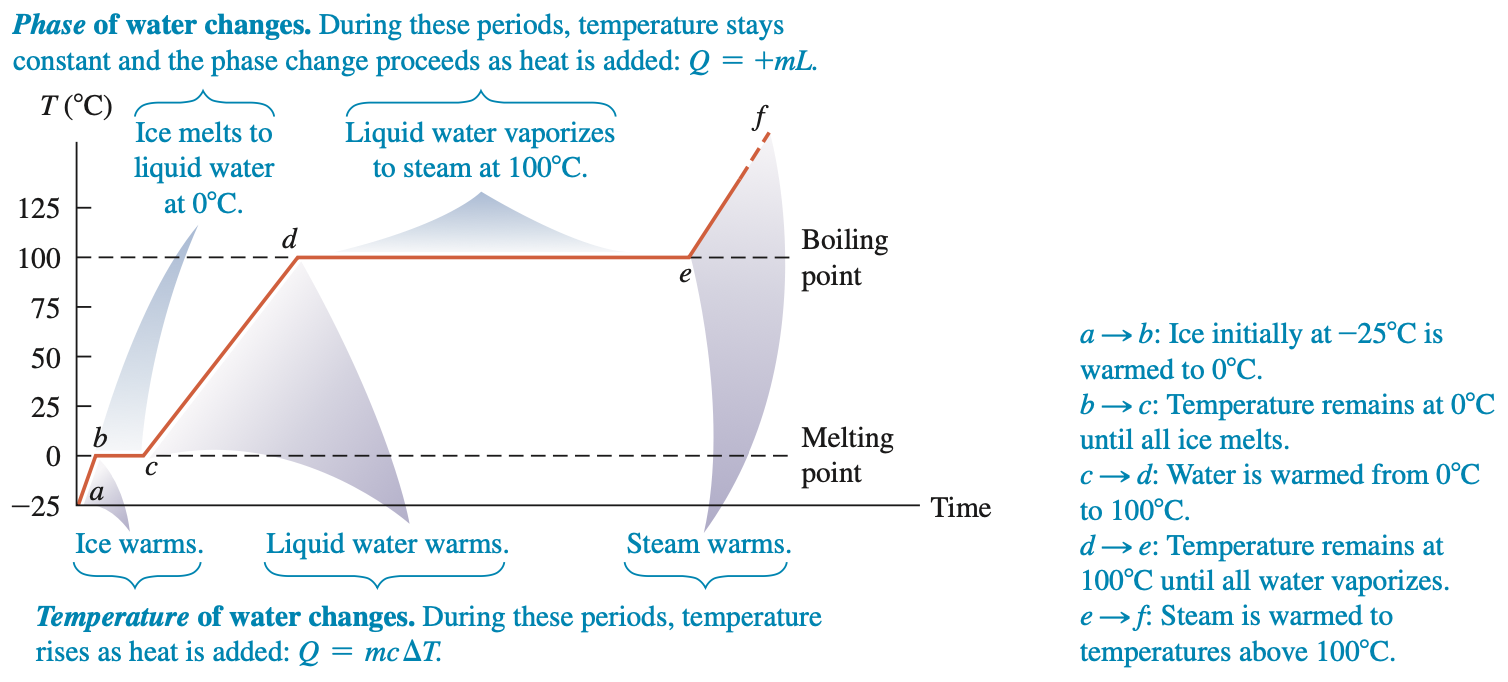
\includegraphics[scale=0.43]{phase-vs-temperature}

\begin{itemize}
  \item The heat transfer required for a material to undergo a phase change is given by \[Q = \pm m L\] where the $\pm$ indicates that heat may need to be added or removed depending on the direction of the phase change (e.g. energy must be added to melt ice), $m$ is the mass of the material, and $L$ is the latent heat associated with the phase change.

  \item When a material is freezing or melting, $L = L_f$ the \textbf{latent heat of fusion}.

  \item When a material is condensing or vaporising, $L = L_v$ the \textbf{latent heat of vaporisation}.

  \item When a material sublimates (changes directly from a solid to a gas, skipping liquid) or deposits/desublimates (changes directly from a gas to a solid, skipping liquid), $L = L_s$ the \textbf{latent heat of sublimation}.

  \item When a material burns, $L = L_c$ the \textbf{latent heat of combustion}.

  \item For any given material at any given pressure, the freezing temperature is the same as the melting temperature. This is called \textbf{phase equilibrium}. Similarly the condensing temperature is the same as the vaporisation temperature.
\end{itemize}

\subsection{Mechanisms of Heat Transfer}

\begin{itemize}
  \item \textbf{Conduction} is a mechanism of heat transfer where the molecules in an area of high temperature have greater kinetic energy, they bump neighboring molecules which increases their kinetic energy, and so on spreading the heat through the material.

  \item The direction of heat flow is always from higher to lower temperature.

  \item When a quantity of heat $dQ$ is transferred through a material in time $dt$ we say the rate of heat flow or the \textbf{heat current} is \[H = \frac{dQ}{dt}.\]

  \item If a rod has cross sectional area $A$, length $L$, one end is held at temperature $T_H$, and the other is held at $T_C$ where $T_H > T_C$, the heat current is \[H = \frac{d Q}{d T} = k A \frac{T_H - T_C}{L}\] where $k$ is the \textbf{thermal conductivity} of the material and $(T_H - T_C) / L$ is the temperature difference per unit length or the magnitude of the \textbf{temperature gradient}.

  \item \textbf{Convection} is the transfer of heat by mass motion of fluid from one region of space to another, e.g. ducted cooling/heating. If the fluid is circulated by a blower or a pump the process is called \textbf{forced convection}; if the flow is caused by differences in density due to thermal expansion, such as hot air rising, the process is called \textbf{free convection}.

  \item \textbf{Radiation} is the transfer of heat by electromagnetic waves such as visible light, infrared, and ultraviolet radiation.

  \item The wavelength of the radiation depends on temperature. At $\qty{20}{\degree C}$ the radiation is infrared. At $\qty{800}{\degree C}$ the radiation is red. At $\qty{3000}{\degree C}$ the radiation is white.

  \item The \textbf{Stefan-Boltzmann law} gives the rate of energy radiation from a surface \[H = A e \sigma T^4\] where $A$ is its surface area, $e$ is a dimensionless constant between 0 and 1 called the \textbf{emissivity} of the surface (1 would be a perfect radiator), $\sigma$ is the \textbf{Stefan-Boltzmann constant} \[\sigma = \qty{5.67037442e-8}{W/(m^2.K^4)},\] and $T$ is the temperature in Kelvin.

  \item An object's surroundings also emit radiation which is absorbed by the object. The net heat current from the object is this \[H = A e \sigma (T^4 - T_s^4)\] where $T_s$ is the temperatue of the surroundings. At thermal equilibrium there is no heat flow.

  \item An object that is a good absorber must also be a good emitter. An ideal radiator with $e = 1$ is also an ideal absorber, absorbing all the raditation that hits it. Such a surface is called an \textbf{ideal black body} or a \textbf{blackbody}.
\end{itemize}

\section{Thermal Properties of Matter}

\subsection{Equations of State}

\begin{itemize}
  \item Quantities such as pressure, volume, temperature, and amount of substance are called \textbf{state variables}.

  \item An equation that relates state variables is called an \textbf{equation of state}.

  \item Molar mass (i.e. the mass of one mole of a substance) is sometimes called \textbf{molecular weight}.

\item The \textbf{ideal gas equation} relates the absolute pressure $p$, volume $V$, number of moles $n$, and absolute temperature (in Kelvin) $T$ \[p V = n R T\] or \[p V = \frac{m_\text{total}}{M} RT\] or \[p V = N k T\] where $R$ is the gas constant \[R = \qty{8.314}{J/(mol.K)}.\]

  \item If the amount of a gas is contant, i.e. $n R$ is constant, then \[\frac{p_1 V_1}{T_1} = \frac{p_2 V_2}{T_2} = \text{constant}.\]

  \item \textbf{Standard temperature and pressure} (STP) is defined as $\qty{0}{\degree C}$ and $\qty{1}{atm}$.

  \item The \textbf{van der Waals} equation extends the ideal gas law to account for the effects of interactions between gas molecules and their finite size \[\left( p + \frac{a n^2}{V^2} \right) (V - n b) = n r T\] where $a$ and $b$ are constants that vary between gases, $a$ depends on the strength of attractive forces between the molecules, and $b$ depends on the volume of the molecules.

  \item A $p V$-diagram is a two-dimensional diagram plotting pressure as a function of volume. Each line, called an \textbf{isotherm}, describes the relationship between pressure and volume at a particular temperature.

  \item In the $p V$-diagrams of non-ideal gases, isotherms can have flat areas. These represent periods where the gas is condensing into a liquid.

  \item The area under a $p V$-curve represents the work done by the system during a volume change.
\end{itemize}

\subsection{Molecular Properties of Matter}

\begin{itemize}
  \item The force between molecules in a gas varies with $r$.

  \item An ideal gas is one whose molecules exert no attractive forces on each other and thus have no potential energy.

  \item The number of molecules in a mole is given by \textbf{Avagadro's number} \[N_A = \num{6.02214076e23} \,\text{molecules}/\text{mol}.\]
\end{itemize}

\subsection{Kinetic-Molecular Model of an Ideal Gas}

\begin{itemize}
  \item The average translational kinetic energy of an ideal gas is \[K_\text{tr} = \frac{3}{2} n R T.\]

  \item The \textbf{Boltzmann constant} is \[k = \frac{R}{N_A} = \num{1.381e-23} \,\text{J}/(\text{molecule K}).\]

  \item The average translational kinetic energy of a gas molecule is \[\frac{1}{2} m (v^2)_\text{av} = \frac{3}{2} kT\] and thus the \textbf{root-mean-square speed} of a gas molecule is \[v_\text{rms} = \sqrt{(v^2)_\text{av}} = \sqrt{\frac{3 k T}{m}} = \sqrt{\frac{3 R T}{M}}\] where $m$ is the mass of a molecule and $M$ is the molar mass.

  \item The average distance travelled by a particle between collisions is called the \textbf{mean free path} \[\lambda = \frac{V}{4 \pi \sqrt{2} r^2 N} = \frac{k T}{4 \pi \sqrt{2} r^2 p}\] where $V$ is the volume of the gas, $r$ is the radius of a gas molecule, $N$ is the number of molecules in the gas, $T$ is its temperature, and $p$ is its volume.
\end{itemize}

\subsection{Heat Capacities}

\begin{itemize}
  \item The \textbf{molar heat capacity at constant volume} of a particular gas is determined by its \textbf{degrees of freedom}, i.e. the number of ways in which it can store kinetic energy.

        \begin{itemize}
          \item Monatomic gases have three degrees of freedom: one for each translational axis.

          \item Diatomic gases have five degrees of freedom: one for each translational axis and two for rotational axes (the third is excluded because it's not affected by collisions).

          \item Polyatomic gases have more than five degrees.
        \end{itemize}

\item The \textbf{principle of equipartition of energy} states that each degree of freedom contributes $\frac{1}{2} k T$ to the average kinetic energy of the gas, i.e. for monatomic gases the average kinetic energy per molecule is $\frac{3}{2} k T$, for diatomic $\frac{5}{2} k T$, etc.

\item The molar heat capacity at constant volume of a gas is equal to \[C_V = \frac{d}{2} R\] where $d$ is the number of degrees of freedom.

  \item Vibrational energy can also contribute to the molar heat capacity at constant volume, but for most diatomic molecules this isn't the case.

  \item Molar heat capacity at constant volume is temperature dependent, with rotational and vibrational degrees of freedom only coming in to play at higher temperatures.

  \item Crystalline solids, i.e. solids whose atoms are arranged in a three-\\dimensional matrix, have six degrees of freedom: three translational and three from the potential energy of intermolecular forces. This results in the \textbf{rule of Dulong and Petit} which states that the molar heat capacity at constant volume of an ideal monatomic solid is \[V_C = 3 R.\]
\end{itemize}

\subsection{Molecular Speeds}

\begin{itemize}
  \item In regards to the speeds of molecules in a gas, a \textbf{distribution function} $f(v)$ gives the probability per unit speed of finding a particle with a speed near $v$. That is, the area under the curve between $f(v_1)$ and $f(v_2)$ gives the probability of finding a particle with speed in that range.

  \item The \textbf{Maxwell-Boltzmann distribution} is a particular distribution\\function \[f(v) = 4 \pi \left( \frac{m}{2 \pi k T} \right)^{3 / 2} v^2 e^{-m v^2 / 2 k T}\] where $m$ is the mass of a molecule, $T$ is the absolute temperature of the gas, and $v$ is the molecular speed.

  \item The peak of the curve and thus the most probable speed occurs at \[v_\text{mp} = \sqrt{\frac{2 k T}{m}}.\]

  \item The average speed is \[v_\text{av} = \sqrt{\frac{8 k T}{\pi m}}.\]

  \item The rms speed is \[v_\text{rms} = \sqrt{\frac{3 k T}{m}}.\]
\end{itemize}

\subsection{Phases of Matter}

\begin{itemize}
  \item A \textbf{$p T$ phase diagram} is a two-dimensional graph with pressure $p$ on the vertical axis and temperature $T$ on the horizontal axis. The plane is separated into three distinct regions: one for each phase of the material (solid, liquid, and gas).

  \item The borders between regions represent points of \textbf{phase equilibrium} where both phases can coexist at the same pressure and temperature.

  \item The \textbf{fusion curve} separates the solid and liquid regions.

  \item The \textbf{vaporisation curve} separates the liquid and gas regions.

  \item The \textbf{sublimation curve} separates the solid and gas regions.

  \item The three curves meet at the \textbf{triple point} — the only conditions under which all three phases can coexist.

  \item The vaporisation curve ends at the \textbf{critical point}. As the pressure and temperature of a substance approaches those of its critical point the physical differences between the liquid and gas phases decrease. At the critical point there are no differences and a substance whose pressure or temperature is gradually decreased won't undergo a phase transition — instead its properties will continuously change from those of a gas to those of a liquid or vice versa.
\end{itemize}

\section{The First Law of Thermodynamics}

\subsection{Thermodynamic Systems}

\begin{itemize}
  \item A \textbf{thermodynamic system} is any collection of objects that is convenient to regard as a unit, and that may have the potential to exchange energy with its surroundings.

  \item A process in which there are changes in the state of a thermodynamic system is called a \textbf{thermodynamic process}.

  \item In a termodynamic process, $Q$ represents the heat added to the system (increasing its energy) and $W$ represents work done by the system on its surroundings (decreasing its energy). Both quantities may be negative in which case they represent heat being removed from the system (decreasing its energy) and the surroundings doing work on the system (increasing its energy), respectively.
\end{itemize}

\subsection{Work Done During Volume Changes}

\begin{itemize}
  \item The work done during a volume change is \[W = \int_{V_1}^{V_2} p \,dV\] where $V_1$ is the initial volume, $V_2$ is the final volume, and $p$ is the pressure.

  \item In the above equation $p$ is often a function of $V$, in which case the integral represents the area under the graph of $p = p(V)$. This is the area under the curve of a $p V$-diagram.

  \item When volume increases, work is positive. When volume decreases, work is negative.
\end{itemize}

\subsection{Paths Between Thermodynamic States}

\begin{itemize}
  \item When a thermodynamic system changes from an initial state to a final state it passes through a series of intermediate states. This series of states is called a \textbf{path}.

  \item There are an infinite number of paths between any given initial and final states, but the amount of work done by the system on its surroundings can differ between paths.

  \item The uncontrolled expansion of a gas into vacuum is called \textbf{free expansion}. The gas does no work as it expands so its temperature doesn't change.
\end{itemize}

\subsection{Internal Energy and the First Law of Thermodynamics}

\begin{itemize}
  \item The \textbf{internal energy} $U$ of a system is the sum of the kinetic energies of all its constituent particles, plus the sum of the potential energies of interactions between these particles.

  \item The \textbf{first law of thermodynamics} states \[\Delta U = Q - W\] where $\Delta U$ is the change in internal energy of a thermodynamic system, $Q$ is the heat added to the system, and $W$ is the work done by the system on its surroundings.

  \item The change in internal energy of a thermodynamic system depends only on its initial and final states, not on the path taken.

  \item A \textbf{cyclic process} is on that starts and ends in the same state. In that case $\Delta U = 0$ and thus $Q = W$: if a net amount of work was done by the system during this process, an equal amount of energy must have flowed into the system as heat $Q$.

  \item In an \textbf{isolated system} that does no work and experiences no heat flow, $Q = W = 0$ and thus $\Delta U = 0$. This means that the inernal energy of an isolated system is constant.

  \item In a cyclic process, the total work is positive if the process moves clockwise around the $p V$-diagram and negative if it moves counterclockwise.

  \item The first law of thermodynamics can also be expressed using infinitesimals \[d U = d Q - d W = d Q - p \,d V.\]
\end{itemize}

\subsection{Kinds of Thermodynamic Processes}

\begin{itemize}
  \item An \textbf{adiabatic process} is one with no heat transfer into or out of the system, i.e. $Q = 0$. This can be achieved by thermally insulating the system or performing the process so quickly that no heat transfer can occur. The path followed by an adiabatic process on a $p V$-diagram is called an \textbf{adiabat}.

  \item An \textbf{isochoric process} is one where the volume of the system doesn't change, i.e. $W = 0$. The path followed by an icochoric process on a $p V$-diagram is called an \textbf{isochor}.

  \item An \textbf{isobaric process} is one where the pressure of the system doesn't change, i.e. $W = p (V_2 - V_1)$. The path followed by an isobaric process on a $p V$-diagram is called an \textbf{isobar}.

  \item An \textbf{isothermal process} is one where the temperature of the system doesn't change. Any heat flowing into or out of the system must occur slowly enough to maintain thermal equilibrium. The path followed by an isothermal process on a $p V$-diagram is called an \textbf{isotherm}.
\end{itemize}

\subsection{Internal Energy of an Ideal Gas}

\begin{itemize}
  \item The internal energy of an ideal gas depends only on its temperature, not on its pressure or volume.
\end{itemize}

\subsection{Heat Capacities of an Ideal Gas}

\begin{itemize}
  \item Gases have two molar heat capacities: one at constant volume $C_V$, and one at constant pressure $C_P$.

  \item When heating a gas at constant pressure, the gas must do work on the container to increase its volume (otherwise pressure would increase). This means not all of the heat is used to increase the temperature of the gas. Thus, the amount of heat required to raise the temperature of a gas at constant pressure is greater than a gas at constant volume, i.e. $C_P > C_V$.

  \item For ideal gases \[C_P = C_V + R.\]

  \item The \textbf{ratio of heat capacities} of a substance is denoted \[\gamma = \frac{C_P}{C_V}.\]

  \item Because the internal energy of an ideal gas depends only on its temperature, not on its pressure or volume, if $\Delta U = n C_V \Delta T$ is valid for one type of process (an isochoric or constant volume process), it must be valid for all other processes.
\end{itemize}

\subsection{Adiabatic Processes for an Ideal Gas}

\begin{itemize}
  \item An adiabatic expansion results in a drop in temperature and an adiabatic compression results in a rise in temperature.

  \item For an adiabatic process \begin{align*}
          T_1 V_1^{\gamma - 1} & = T_2 V_2^{\gamma - 1}                     \\ \\
          p_1 V_1^\gamma       & = p_2 V_2^\gamma                           \\ \\
          W                    & = n C_V (T_1 - T_2)                        \\ \\
          W                    & = \frac{C_V}{R} (p_1 V_1 - p_2 V_2)        \\
                               & = \frac{1}{\gamma - 1} (p_1 V_1 - p_2 V_2)
        \end{align*}
\end{itemize}

\section{The Second Law of Thermodynamics}

\subsection{Directions of Thermodynamic Processes}

\begin{itemize}
  \item Thermodynamic processes that occur between objects that aren't in thermodynamic equilibrium are irreversible, e.g. heat flowing from an area of higher to lower temperature, free expansion of gas, etc.

  \item Thermodynamic processes that occur between objects that are very nearly in thermodynamic equilibrium approach being reversible. They are also called \textbf{equilibrium processes}.
\end{itemize}

\subsection{Heat Engines}

\begin{itemize}
  \item Any device that transforms heat into work or mechanical energy is called a \textbf{heat engine}.

  \item Usually a quantity of matter inside the engine undergoes inflow and outflow of heat, expansion and compression, and sometimes change of phase. We call this matter the \textbf{working substance} of the engine.

  \item All heat engines absorb heat from a \textbf{hot reservoir} and discard waste heat to a \textbf{cold reservoir}.

  \item The amount of heat absorbed from the hot reservoir is denoted $Q_H$ (positive) and the amount of heat discarded to the cold reservoir is denoted $Q_C$ (negative).

  \item If a heat engine undergoes a cyclic process $\Delta U = 0$ so \[W = Q = Q_H + Q_C = |Q_H| - |Q_C|.\]

  \item The \textbf{thermal efficiency} of a heat engine \[e = \frac{W}{Q_H} = 1 + \frac{Q_C}{Q_H} = 1 - \left| \frac{Q_C}{Q_H} \right|\] represents the fraction of input energy that's converted into useful work.
\end{itemize}

\subsection{Internal Combustion Engines}

\begin{itemize}
  \item The \textbf{Otto cycle} is an idealised version of the thermodynamic process inside a gasoline engine.

  \item The thermal efficiency of the Otto cycle is \[e = 1- \frac{1}{r^{\gamma - 1}}\] where $r$ is the compression ratio of the engine.
\end{itemize}

\subsection{Refigerators}

\begin{itemize}
  \item A fridge is like a reverse heat engine — it takes heat from a cold place (the inside of the fridge) to a hot place (the outside of the fridge). However, where a heat engine has a net output of work a fridge has a net input of work.

  \item When modelling a fridge as a thermodynamic system, $Q_C$ is positive, $Q_H$ is negative, and $W$ is negative.

  \item A more performant fridge will maximise $Q_C$ (the heat removed from the inside of the fridge) for a given $W$ (the power input to the fridge). This is captured by the \textbf{coefficient of performance} \[K = \frac{|Q_C|}{|W|} = \frac{|Q_C|}{|Q_H| - |Q_C|}.\]

  \item Another way of thinking about the performance of an air conditioner or fridge is in terms of the amount of heat removed per unit time, i.e. the heat current $H$, and the energy input per unit time, i.e. the power $P$. In terms of these units the coefficient of performance is \[K = \frac{|Q_C|}{|W|} = \frac{H t}{P t} = \frac{H}{P}.\]
\end{itemize}

\subsection{The Second Law of Thermodynamics}

\begin{itemize}
  \item The \textbf{second law of thermodynamics} states that it is impossible for any system to undergo a process in which it absorbs heat from a reservoir at a single temperature and converts the heat completely into mechanical work, with the system ending in the same state in which it began.

  \item An alternative wording is that it is impossible for any process to have as its sole result the transfer of heat from a cooler to a hotter object.
\end{itemize}

\subsection{The Carnot Cycle}

\begin{itemize}
  \item The \textbf{Carnot cycle} is an ideal thermodynamic process that provides an upper limit on the maximum efficiency of an engine. In it, only reversible thermodynamic processes may be used — namely adiabatic and isothermal processes.
\end{itemize}

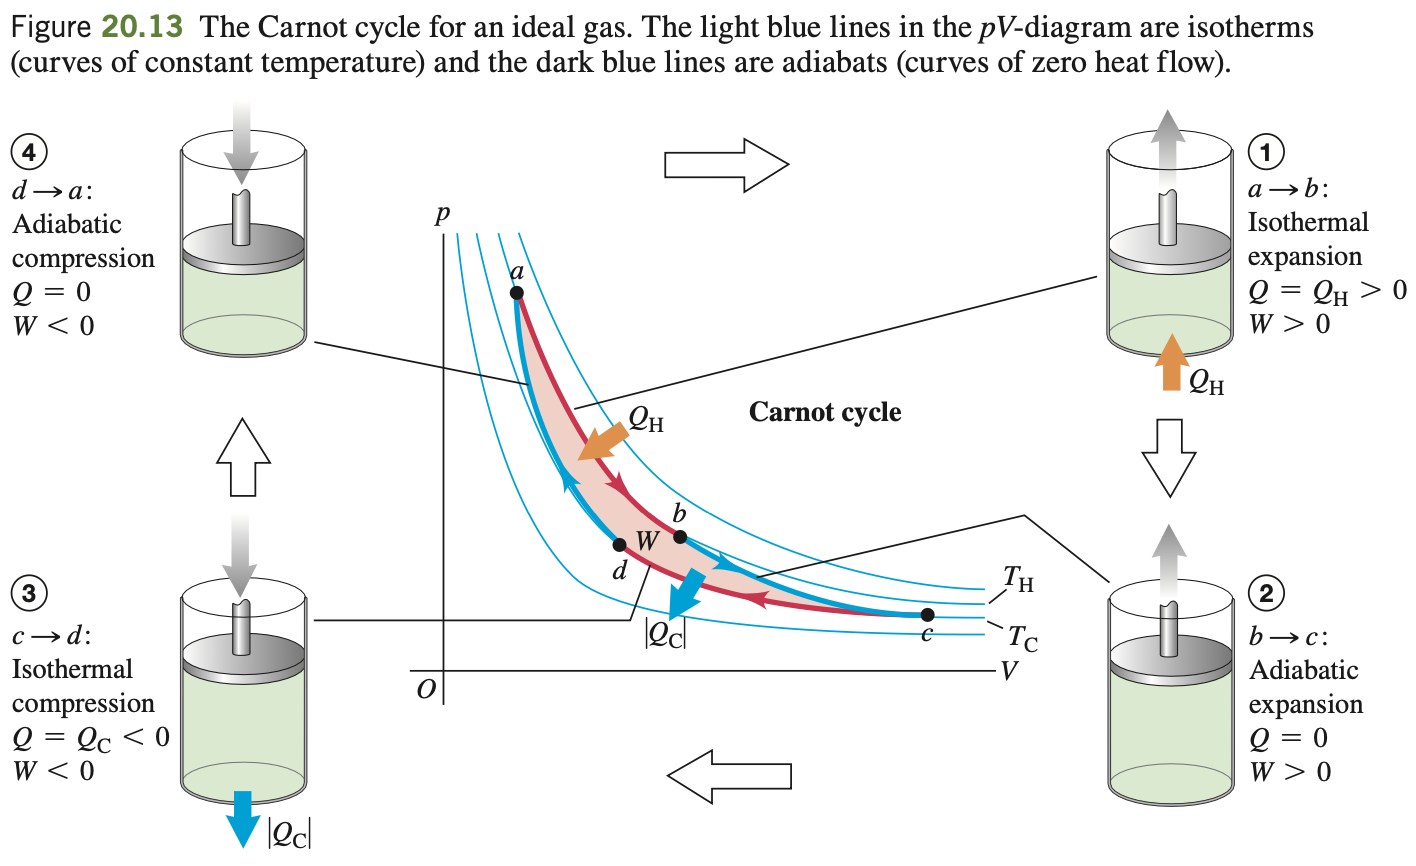
\includegraphics[scale=0.464]{carnot-cycle}

\begin{itemize}
  \item The amount of heat transferred to/from the reservoirs in a Carnot cycle are related to the temperatures of the reservoirs by \[\frac{Q_C}{Q_H} = -\frac{T_C}{T_H}.\]

  \item The efficiency of a Carnot engine is \[e_\text{Carnot} = 1 - \frac{T_C}{T_H}.\]

  \item Because all processes in the Carnot cycle are reversible, the cycle itself can be reversed to make a Carnot fridge.

  \item The coefficient of performance of a Carnot fridge is \[K_\text{Carnot} = \frac{T_C}{T_H - T_C}.\]
\end{itemize}

\subsection{Entropy}

\begin{itemize}
  \item \textbf{Entropy} $S$ is a measure of the randomness in a system. When you add heat to a system the constituent particles gain kinetic energy, there is more randomness to their positions, and thus entropy increases. When you remove heat from a system entropy decreases.

  \item The units of entropy are $\unit{J/K}$.

  \item The change in entropy during a reversible isothermal process is \[\Delta S = \frac{Q}{T}.\]

  \item The change in entropy during any reversible thermodynamic process can be calculated as \[\Delta S = \int_1^2 \frac{d Q}{T}\] where $\Delta S$ is the change in entropy, $1$ is the initial state, $2$ is the final state, $d Q$ is the infinitesimal heat flow into the system, and $T$ is the absolute temperature of the system.

  \item Entropy is determined entirely by the state of a system, not how it got there, i.e. entropy is path independent.

  \item In an adiabatic process $Q = 0$ and thus there is no change in entropy.

  \item To calculate the change in entropy of an irreversible process, come up with a series of reversible processes that take the system between the same states and calculate the change in entropy of that.

  \item When a system undergoes a reversible change from state $a$ to state $b$, the change in entropy is $0$. This means that the change in entropy of adiabatic and isothermal processes are $0$ (because they are reversible). The Carnot cycle is composed of adiabatic and isothermal processes so its change in entropy is also $0$. In general, the change in entropy for any reversible cyclic process is $0$.

  \item An alternative formulation of the second law of thermodynamics is that no process is possible in which total entropy decreases, when all systems that take part in the process are included.
\end{itemize}

\subsection{Microscopic Interpretation of Entropy}

\begin{itemize}
  \item A description of the \textbf{macroscopic state} of a system describes the system as a whole rather than individual components of the system, e.g. ``50\% of the coins are heads, 50\% are tails.''

  \item A description of the \textbf{microscopic state} of a system describes the individual components, e.g. ``Coin 1 is heads, coin 2 is tails, etc.''

  \item Many microscopic states may correspond to a given macroscopic state.

  \item For any thermodynamic system, the most probable macroscopic state is the one with the greatest number of corresponding microscopic states, which is also the macroscopic state with the greatest randomness and the greatest entropy.

  \item The entropy of a given macroscopic state is \[S = k \ln w\] where $k$ is the Boltzmann constant and $w$ is the number of microscopic states associated with the macroscopic state.
\end{itemize}

\setcounter{section}{36}
\section{Relativity}

\subsection{Invariance of Physical Laws}

\begin{itemize}
  \item \textbf{Einstein's first postulate} or the \textbf{principle of relativity} states that the law of physics are the same in every inertial frame of reference.

  \item \textbf{Einstein's second postulate} states that the speed of light in vacuum is the same in all intertial frames of reference and is independent of the motion of the source.

  \item It is not possible to travel at the speed of light.

  \item A \textbf{Galilean transformation} transforms between the coordinates of two reference frames that differ only by constant relative motion, e.g. \begin{align*}
          x & = x' + v t \\
          y & = y'       \\
          z & = z'.
        \end{align*}
\end{itemize}

\subsection{Relativity of Simultaneity}

\begin{itemize}
  \item In a given frame of reference an \textbf{event} is an occurence that has a definite position and time.

  \item In general, two events that are \textbf{simultaneous} in one frame of reference are not simultaneous in another frame that is moving relative to the first, even if both are inertial frames.
\end{itemize}

\subsection{Relativity of Time Intervals}

\begin{itemize}
  \item There is only one reference frame in which a given point is at rest and we call it the point's \textbf{rest frame}.

  \item The time interval measured between two events that occur at the same point (and thus in the point's reference frame) is called \textbf{proper time $\Delta t_0$}.

  \item The time interval between those two same events in another frame of reference moving at speed $u$ relative to the rest frame is \[\Delta t = \frac{\Delta t_0}{\sqrt{1 - u^2 / c^2}}\] which is greater than $\Delta t_0$. This phenomenon is called \textbf{time dilation}.

  \item The \textbf{Lorentz factor} is defined as \[\gamma = \frac{1}{\sqrt{1 - u^2 / c^2}}.\]

  \item If the relative speed $u$ of a reference frame is large enough that the Lorentz factor $\gamma$ is appreciably greater than $1$, the speed is said to be \textbf{relativistic}. Otherwise it's said to be \textbf{nonrelativistic}.
\end{itemize}

\subsection{Relativity of Length}

\begin{itemize}
  \item The length of a body as measured in its rest frame is called its \textbf{proper length $l_0$}.

  \item In a moving reference frame, The length of a body in the direction parellel to motion is \[l = \frac{l_0}{\gamma}\] which is less than $l_0$. This phenomenon is called \textbf{length contraction}.

  \item Length contraction doesn't occur in directions perpendicular to motion.
\end{itemize}

\subsection{The Lorentz Transformations}

\begin{itemize}
  \item If $S'$ is a reference frame moving at speed $u$ along the $x$-axis relative to reference frame $S$, then the \textbf{Lorentz transformation} can be used to determine the spacetime coordinates $x'$, $y'$, $z'$, and $t'$ in $S'$ from coordinates $x$, $y$, $z$, and $t$ in $S$ \begin{align*}
          x' & = \frac{x - u t}{\sqrt{1 - u^2 / c^2}} = \gamma (x - u t)              \\
          y' & = y                                                                    \\
          z' & = z                                                                    \\
          t' & = \frac{t - u x / c^2}{\sqrt{1 - u^2 / c^2}} = \gamma (t - u x / c^2).
        \end{align*}

  \item At relativistic speeds length and time have no meaning independent of a reference frame, so we use \textbf{spacetime coordinates} $x$, $y$, $z$, and $t$.

  \item The \textbf{Lorentz velocity transformation} can be used to determine the velocity in $S'$ in terms of the velocity in $S$ \[v_x' = \frac{v_x - u}{1 - u v_x / c^2}.\]
\end{itemize}

\subsection{The Doppler Effect For Electromagnetic Waves}

\begin{itemize}
  \item When the source of an electromagnetic wave of proper frequency $f_0$ is approaching a stationary observer at speed $u$, the observer measures frequency \[f = \sqrt{\frac{c + u}{c - u}} f_0.\] When the source is moving away from the observer the sign of $u$ changes.
\end{itemize}

\subsection{Relativistic Momentum}

\begin{itemize}
  \item The mass of a particle when it is at rest relative to the observer is called its \textbf{rest mass}.

  \item A particle's \textbf{relativistic momentum} is \[\mathbf{p} = \frac{m \mathbf{v}}{\sqrt{1 - v^2 / c^2}} = \gamma m \mathbf{v}.\] This means that as a particle's speed increases so does its relativistic momentum.

  \item The expression $\gamma m$ is sometimes called the \textbf{relativistic mass}, which increases with a particle's speed.

  \item Newton's second law must be adjusted at relativistic speeds. For forces parallel to the direction of motion \[F = \gamma^3 m a\] and for forces perpendicular to the direction of motion \[F = \gamma m a.\] This means that, unless the net force on a particle moving at relativistic speeds is either parallel or perpendicular to its direction of motion, the acceleration and force vectors aren't parallel.
\end{itemize}

\subsection{Relativistic Work and Energy}

\begin{itemize}
  \item The kinetic energy of a particle travelling at relativistic speeds is \[K = (\gamma - 1) m c^2.\]

  \item The total energy of a particle is \[E = \gamma m c^2\] or \[E^2 = (m c^2)^2 + (p c)^2.\]

  \item For a particle at rest $E = m c^2$. This is called the particle's \textbf{rest energy}.
\end{itemize}

\section{Photons: Light Waves Behaving as Particles}

\subsection{Light Absorbed as Photons: The Photoelectric Effect}

\begin{itemize}
  \item To escape from the surface of a material, an electron must absorb enough energy to overcome the attraction of positive ions in the material. The \textbf{photoelectric effect} is the phenomenon where light gives the electroncs this energy, producing a current.

  \item The maximum kinetic energy of an electron emitted via the photoelectric effect is \[K = \frac{1}{2} m v_\text{max}^2 = e V_0\] where $V_0$ is the \textbf{stopping potential}, i.e. the potential diffreence between the anode and cathode at which electrons no longer flow.

  \item The energy of a photon is \[E = h f = \frac{h c}{\lambda}\] where $h$ is \textbf{Planck's constant} \[h = \qty{6.62606957e-34}{J.s}.\]

  \item The maximum kinetic energy of an electron emitted via the photoelectric effect is \[e V_0 = h f - \phi\] where $\phi$ is the material's \textbf{work function}, i.e. the amount of energy required for an electron to overcome the attractive foces of ions.

  \item The momentum of a photon is \[p = \frac{E}{c} = \frac{h f}{c} = \frac{h}{\lambda}.\]
\end{itemize}

\subsection{Light Emitted as Photons: X-Ray Production}

\begin{itemize}
  \item Accelerated charges produce electromagnetic waves. When an electron is ``braked'' by a material it is decelerated, producing an electromagnetic wave. The frequency of that wave is determined by the charge's kinetic energy. If the charge is accelerated across a potential difference of $V$ then \[K = e V = h f = \frac{h c}{\lambda}.\]
\end{itemize}

\subsection{Light Scattered as Photons: Compton Scattering\\and Pair Production}

\begin{itemize}
  \item When a photon strikes an electron it gives up some of its energy and momentum to the electron and is redirected at an angle $\phi$ from its original path. The change in wavelength of the photon is given by \[\lambda' - \lambda = \frac{h}{m c} (1 - \cos \phi)\] where $\lambda'$ is the wavelength of the scattered photon, $\lambda$ is the original wavelength of the photon, $h$ is Planck's constant, $m$ is the mass of the electron, $c$ is the speed of light in vacuum, and $\phi$ is the scattering angle.

  \item If a gamma ray photon is fired at a target, it may not scatter. Instead it may disappear and be replaced with an electron / positron pair. A \textbf{positron} is a particle with the same mass as an electron but with opposite charge ($+e$).
\end{itemize}

\subsection{Wave-Particle Duality, Probability, and Uncertainty}

\begin{itemize}
  \item The \textbf{Heisenberg uncertainty principle} states that it is impossible to simultaneously determine both the position and momentum of a particle with arbitrarily great precision \[\Delta x \Delta p_x \ge \hbar / 2\] where $\Delta x$ is uncertainty in the $x$ coordinate, $\Delta p_x$ is uncertainty in the $x$ momentum, and $\hbar$ is Planck's constant divided by $2 \pi$.

  \item The Heisenberg uncertainty principle for energy and time is \[\Delta t \Delta E \ge \hbar / 2.\]
\end{itemize}

\section{Particles Behaving as Waves}

\subsection{Electron Waves}

\begin{itemize}
  \item Like light acting like a particle, particles can act like a wave. The \textbf{de Broglie wavelength} of a particle travelling at non-relativistic speed is \[\lambda = \frac{h}{p} = \frac{h}{mv}.\] At relativistic speed we replace $p$ with $\gamma p$ \[\lambda = \frac{h}{\gamma p} = \frac{h}{\gamma m v}.\]

  \item The energy of a particle is related to its frequency in the same way as light \[E = h f.\]

  \item The de Broglie wavelength of an electron accelerated through a potential difference $V_{b a}$ is \[\lambda = \frac{h}{p} = \frac{h}{\sqrt{2 m e V_{b a}}}.\]
\end{itemize}

\subsection{The Nuclear Atom and Atomic Spectra}

\begin{itemize}
  \item Heated materials emit light and different materials emit different kinds of light. If we pass this light through a prism or diffraction grating we can separate the light into its component wavelengths. This is called an \textbf{emission line spectrum} and the lines are called \textbf{spectral lines}.

  \item Solids and liquids have continuous emission line spectrums, i.e. they emit all wavelengths of visible light, while gases only emit a subset of wavelengths.

  \item The emission line spectrum of each element is constant.

  \item While a heated gas selectively emits certain wavelengths of light, a cooled gas selectively absorbs the same wavelengths. If we pass white light onto the material and observe the transmitted (i.e. not absorbed) wavelengths we can determine which wavelengths were absorbed. This is called the gas's \textbf{absorption line spectrum}.
\end{itemize}

\subsection{Energy Levels and the Bohr Model of the Atom}

\begin{itemize}
  \item An atom's internal energy may be equal to a set of possible \textbf{energy levels}, but not to an amount of energy between these levels.

  \item An atom's lowest energy level is known as its \textbf{ground state} and higher energy levels are known as \textbf{excited states}.

  \item When an atom drops from a higher to a lower energy level it emits a photon whose energy is equal to the difference between the energy levels \[h f = \frac{h c}{\lambda} = E_\text{i} - E_\text{f}.\]

  \item An atom can be raised from a lower to a higher energy level via collisions or absorption of photons, however the photon's energy must be equal to the different between the energy levels.

  \item If an atom is in its ground state there are limited wavelengths of photons it can absorb, i.e. only those whose energy is equal to that of the higher energy levels. However, when the atom is emitting photons it has more options as it can go between different higher energy levels. This means atoms can emit longer wavelengths than they absorb, e.g. absorb infrared and emit visible, a process called \textbf{fluorescence}.

  \item The magnitude of an electron's angular momentum is quantized and must be an integer multiple of $\hbar$, i.e. \[L_n = m v_n r_n = n \hbar\] where $m$ is the mass of the electron, $v_n$ is its speed in orbit number $n$, $r_n$ is its radius in orbit number $n$, and $n = 1, 2, 3, \ldots$ is called the \textbf{principle quantum number} of the orbit.

  \item Electrons can be considered particles orbiting the nucleus or standing waves at the same radius as the particle. The circumference of the orbit must be equal to an integer multiple of the wavelength of the standing wave.

  \item Under the Bohr model, the radius of the $n$th orbit is \[r_n = \epsilon_0 \frac{n^2 h^2}{\pi m e^2} = n^2 a_0\] where $a_0$ is the \textbf{Bohr radius} and the orbital speed of the $n$th orbit is \[v_n = \frac{1}{\epsilon_0} \frac{e^2}{2 n h}.\]

  \item The total energy of an electron is \[E_n = -\frac{h c R}{n^2}\] where \[R = \frac{m e^4}{8 \epsilon_0^2 h^3 c} = \qty{1.097e7}{m^{-1}}\] is called the \textbf{Rydberg constant}.

  \item The energy required to ionise an atom, i.e. remove an electron, is the energy required to move the electron from the ground state ($n = 1$) to an infinitely large orbit radius equal to \[E_\infty - E_1 = 0 - E_1 = -E_1.\] This value is positive because $E_1$ is negative.

  \item The Bohr model predicts emission and absorption spectrums with $0.1\%$ accuracy. The discrepancy comes from the assumption that the nucleus doesn't move. It can be made more accurate by using the atom's \textbf{reduced mass} \[m_r = \frac{m_1 m_2}{m_1 + m_2}\] instead of the electron's mass.

  \item The Bohr model can be extended to other one-electron atoms, called \textbf{hydrogenlike atoms}. In such atoms the nucleur charge isn't $e$ but $Z e$ where $Z$ is the atomic number, i.e. the number of protons in the nucleus. This means we must replace $e^2$ with $Z e^2$ in the formulas above.
\end{itemize}

\subsection{The Laser}

\begin{itemize}
  \item The number of atoms at a given energy level is given by \[n = A e^{-E / k T}\] where $A$ is a constant determined by the total number of atoms in the gas.
\end{itemize}

\subsection{Continuous Spectra}

\begin{itemize}
  \item A hypothetical material that absorbs all wavelengths of light is called a \textbf{blackbody}. Because materials' absorption and emission spectra are equal, the material would also emit all wavelengths of light when heated.

  \item The \textbf{Stefan-Boltzmann law} gives the intensity of radiation per unit area from a blackbody \[I = \sigma T^4\] where $\sigma$ is the Stefan-Boltzmann constant and $T$ is the absolute temperature of the blackbody. This differs from the Stefan-Boltzmann law in section 17.7 in that $A$ isn't included because the intensity is per unit area and $e$ isn't included because it's a blackbody and $e = 1$.

  \item The intensity of emitted radiation is not equal across all wavelengths and can be described by the intensity per wavelength interval $I(\lambda)$ called the \textbf{spectral emittance}. The intensity corresponding to wavelengths in the interval $[\lambda, \lambda + d \lambda]$ is thus given by $I(\lambda) \,d\lambda$.

\item The spectral emittance $I(\lambda)$ differs based on temperature $T$ and has a peak wavelength $\lambda_m$ where the intensity per unit wavelength is the greatest. The \textbf{Wien displacement law} relates these two quantities \[\lambda_m T = \qty{2.90e-3}{m.K}.\]

  \item \textbf{Planck's radiation law} gives the spectral emittance (intensity per unit wavelength) of a blackbody \[I(\lambda) = \frac{2 \pi h c^2}{\lambda^5 (e^{h c / \lambda k T} - 1)}.\]
\end{itemize}

\section{Quantum Mechanics I: Wave Functions}

\subsection{Wave Functions and the One-Dimensional\\Schrödinger Equation}

\begin{itemize}
  \item A \textbf{free particle} is a particle that experiences no force, i.e. its potential energy function is $0$ at all locations.

  \item Thus the energy of a free particle is equal to its kinetic energy \[E = K = \frac{1}{2} m v^2 = \frac{m^2 v^2}{2 m} = \frac{p^2}{2 m}.\]

  \item From the de Broglie relationships we find \begin{align*}
          E & = h f = \frac{h}{2 \pi} 2 \pi f = \hbar \omega                         \\
          p & = \frac{h}{\lambda} = \frac{h}{2 \pi} \frac{2 \pi}{\lambda} = \hbar k.
        \end{align*}

  \item Substituting these equations into that of the energy of a free particle we find \[\hbar \omega = \frac{\hbar^2 k^2}{2 m}.\]

\item The \textbf{one-dimensional Schrödinger equation for a free particle} is \[-\frac{\hbar^2}{2 m} \frac{\partial^2 \Psi(x, t)}{\partial x^2} = i \hbar \frac{\partial \Psi(x, t)}{\partial t}\] the general solution of which is \[\Psi(x, t) =  A[\cos (k x - \omega t) + i \sin (k x - \omega t)] = A e^{i (k x - \omega t)}.\]

  \item For a particle that can only move in the $x$ direction, $|\Psi(x, t)|^2$ is called the \textbf{probability distribution function} and the value $|\Psi(x, t)|^2 \,dx$ is the probability that the particle will be found at time $t$ at a coordinate between $x$ and $x + dx$. This requires that the wave function $\Psi$ be normalized, i.e. \[\int_{-\infty}^\infty |\Psi(x, t)|^2 \,dx = 1.\]

  \item The probability distribution function can be calculated by multiplying $\Psi(x, t)$ buy its complex conjugate \[\Psi(x, y)|^2 = \Psi(x, t) \Psi^*(x, t).\]

  \item A localised wave pulse constructed from multiple superposed waves is called a \textbf{wave packet} and it has properties of both a particle and a wave. It can be represented by an expression like \[\Psi(x, t) = \int_{-\infty}^\infty A(k) e^{i (k x - \omega t)} \,dk.\]

  \item The \textbf{general one-dimensional Schrödinger equation}, i.e. for a particle with a nonzero potential energy function $U(x)$, is \[-\frac{\hbar^2}{2 m} \frac{\partial^2 \Psi(x, t)}{\partial x^2} + U(x) \Psi(x, t) = i \hbar \frac{\partial \Psi(x, t)}{\partial t}.\] If $\Psi(x, t) = A e^{i (k x - \omega t)}$ this reduces to \begin{align*}
          -\frac{\hbar^2}{2 m} (-k^2 \Psi(x, t)) + U(x) \Psi(x, t) & = i \hbar (-i \omega \Psi(x, t)) \\
          \frac{\hbar^2 k^2}{2 m} \Psi(x, t) + U(x) \Psi(x, t)     & = \hbar \omega \Psi(x, t)        \\
          \frac{\hbar^2 k^2}{2 m} + U(x)                           & = \hbar \omega                   \\
          K + U(x)                                                 & = E.
        \end{align*}

  \item If a particle has a known energy $E$ then $\omega = E / \hbar$ and the wave function can be written as \[\Psi(x, t) = A e^{i (k x - E t / \hbar)} = A e^{i k x} e^{-i E t / \hbar} = \psi(x) e^{-i E t / \hbar}.\] This is known as the \textbf{time-dependent wave function for a state of definite energy} or a \textbf{stationary state} because \begin{align*}
          |\Psi(x, t)|^2 & = \Psi(x, t) \Psi(x, t)^*                                    \\
                         & = (\psi(x) e^{-i E t / \hbar}) (\psi^*(x) E^{i E t / \hbar}) \\
                         & = \psi(x) \psi^*(x)                                          \\
                         & = |\psi(x)|^2,
        \end{align*} i.e. the probability distribution function does not depend on time.

  \item Substituting the stationary state equation into the Schrödinger equation we find the \textbf{time-independent one-dimensional Schrödinger equation} \[-\frac{\hbar^2}{2 m} \frac{d^2 \psi(x)}{d x^2} + U(x) \psi(x) = E \psi(x).\]
\end{itemize}

\subsection{Particle in a Box}

\begin{itemize}
  \item For a particle confined to a potential well, i.e. \[U(x) = \begin{cases}
            \infty & x \le 0   \\
            0      & 0 < x < L \\
            \infty & L \le x
          \end{cases}\] the stationary state wave function between $x = 0$ and $x = L$ must satisfy the time-indepdendent one-dimensional Schrödinger equation \[-\frac{\hbar}{2 m} \frac{d^2 \psi(x)}{d x^2} = E \psi(x)\] and the boundary conditions $\psi(0) = 0$ and $\psi(L) = 0$.

  \item The general solution to the above is \begin{align*}
          \psi(x) & = A_1 e^{i k x} + A_2 e^{-i k x} \\
                  & = 2 i A_1 \sin k x               \\
                  & = C \sin k x
        \end{align*} where $k = n \pi / L$ and $\lambda = 2 \pi / k = 2 L / n$ for $n = 1, 2, 3, \ldots$ which is the same as a standing wave one a string.

  \item For each quantum number $n$, a particle in a box has a wavelength \[\lambda_n = \frac{2 L}{n}\] and thus a momentum \[p_n = \frac{h}{\lambda_n} = \frac{n h}{2 L}\] and an energy \[E_n = \frac{p_n^2}{2 m} = \frac{n^2 h^2}{8 m L^2} = \frac{n^2 \pi^2 \hbar^2}{2 m L^2}.\]

  \item Each energy level has an associated wave function \[\psi_n(x) = C \sin \frac{n \pi x}{L}.\]

  \item A particle in a box cannot have zero energy because that implies zero uncertainty in momentum and, by Hiesenberg's uncertainty principle, infinite uncertainty in position which potentially places the particle outside the box.

\item The normalized time-independent wave function for a particle in a box is \[\psi_n(x) = \sqrt{\frac{2}{L}} \sin \frac{n \pi x}{L}.\]
\end{itemize}

\subsection{Potential Wells}

\begin{itemize}
  \item A \textbf{potential well} is a potential-energy function $U(x)$ that has a minimum.

  \item A \textbf{finite well} is a potential well that has straight sides but finite height: \[U(x) = \begin{cases}
            U_0 & x \le 0   \\
            0   & 0 < x < L \\
            U_0 & L \le x
          \end{cases}.\]

  \item In Newtonian mechanics a particle is trapped in a potential well if its total energy $E$ is less than $U_0$. In quantum mechanics, such a trapped state is called a \textbf{bound state}.

  \item The wave function for a particle in a finite well of depth $U_0$ and width $L$ is \[\psi(x) = \begin{cases}
            C e^{\kappa x}                                                                                          & x \le 0   \\
            A \cos \left( \frac{\sqrt{2 m E}}{\hbar} x \right) + B \sin \left( \frac{\sqrt{2 m E}}{\hbar} x \right) & 0 < x < L \\
            D e^{-\kappa x}                                                                                         & L \le x
          \end{cases}\] where $\kappa = \sqrt{2 m (U_0 - E)} / \hbar$.
\end{itemize}

\subsection{Potential Barriers and Tunneling}

\begin{itemize}
  \item A \textbf{potential barrier} is a potential ene rgy function with a maximum.

  \item The \textbf{tunneling probability} $T$ is the probability a particle tunnels\\through a potential barrier and is equal to \[T = G e^{-2 \kappa L}\] where \[G = 16 \frac{E}{U_0} \left( 1 - \frac{E}{U_0} \right)\] and \[\kappa = \frac{\sqrt{2 m (U_0 - E)}}{\hbar}.\]
\end{itemize}

\subsection{The Harmonic Oscilator}

\begin{itemize}
  \item The energy levels for a harmonic oscillator are \[E_n = \left( n + \frac{1}{2} \right) \hbar \sqrt{\frac{k'}{m}} = \left( n + \frac{1}{2} \right) \hbar \omega, n = 0, 1, 2, \ldots\] where $n$ is the quantum number (where $n = 0$ is the ground state), $k'$ is the potential well's force constant, and $\omega$ is the oscillator's angular frequency.
\end{itemize}

\section{Quantum Mechanics II: Atomic Structure}

\subsection{The Schrödinger Equation in Three Dimensions}

\begin{itemize}
  \item The general form of the Schrödinger equation in three dimensions is \begin{align*}
           & -\frac{\hbar^2}{2 m} \left( \frac{\partial^2 \Psi(x, y, z, t)}{\partial x^2} + \frac{\partial^2 \Psi(x, y, z, t)}{\partial y^2} + \frac{\partial^2 \Psi(x, y, z, t)}{\partial z^2} \right) \\
           & \qquad + U(x, y, z) \Psi(x, y, z, t) = i \hbar \frac{\partial \Psi(x, y, z, t)}{\partial t}
        \end{align*}

  \item As in one dimension, the square of the modulus of the wave function is the probability distribution function of the particle's location, i.e. the probability of finding the particle in a volume $V$ is given by \[\int_V |\Psi(x, y, z, t)|^2 \,dV.\]

  \item The normalization condition on the wave function is that the integral of its modulus squared over all space must equal $1$, i.e. the probability that the particle is somewhere is $1$ \[\int |\Psi(x, y, z, t)|^2 \,dV = 1.\]

  \item If the wave function represents a state of definite energy $E$ the time component can be dropped leaving the time-independent three-dimensional Schrödinger equation \begin{align*}
           & -\frac{\hbar^2}{2 m} \left( \frac{\partial^2 \psi(x, y, z)}{\partial x^2} + \frac{\partial^2 \psi(x, y, z)}{\partial y^2} + \frac{\partial^2 \psi(x, y, z)}{\partial z^2} \right) \\
           & \qquad + U(x, y, z) \psi(x, y, z) = E \psi(x, y, z).
        \end{align*}

  \item The probability distribution function for a stationary state in three dimensions is \[|\psi(x, y, z)|^2\] giving the normalization condition \[\int |\psi(x, y, z)|^2 \,dV = 1.\]
\end{itemize}

\subsection{Particle in a Three-Dimensional Box}

\begin{itemize}
  \item The time-independent Schrödinger equation in three dimensions reduces to three independent equations — one for each dimension. These equations are the same as for a particle in a one-dimensional box. The solutions for each dimension are thus \begin{align*}
          X_{n_X}(x) & = C_X \sin \frac{n_X \pi x}{L} & (n_X = 1, 2, 3, \ldots) \\
          Y_{n_Y}(y) & = C_Y \sin \frac{n_Y \pi y}{L} & (n_Y = 1, 2, 3, \ldots) \\
          Z_{n_Z}(z) & = C_Z \sin \frac{n_Z \pi z}{L} & (n_Z = 1, 2, 3, \ldots)
        \end{align*} where $C_X$, $C_Y$, and $C_Z$ are constants.

  \item This means that there are three different quantum numbers — one for each dimension — and the ``dead spots'' of the wave function are determined by these numbers.

  \item The energy of the particle is $E = E_X + E_Y + E_Z$ where \begin{align*}
          E_X = \frac{n_X^2 \pi^2 \hbar^2}{2 m L^2} & (n_X = 1, 2, 3, \ldots)  \\
          E_Y = \frac{n_Y^2 \pi^2 \hbar^2}{2 m L^2} & (n_Y = 1, 2, 3, \ldots)  \\
          E_Z = \frac{n_Z^2 \pi^2 \hbar^2}{2 m L^2} & (n_Z = 1, 2, 3, \ldots).
        \end{align*} Equivalently \[E_{n_X,n_Y,n_Z} = \frac{(n_X^2 + n_Y^2 + n_Z^2) \pi^2 \hbar^2}{2 m L^2}.\]

  \item For quantum systems in multiple dimensions, two or more sets of quantum numbers (and thus quantum states) can correspond to the same energy level. This is called \textbf{degeneracy} and the quantum states are said to be \textbf{degenerate}.

  \item For a particle in a three-dimensional box, degeneracy is a result of the sides of the box having equal lengths. The degeneracy can be removed by making the sides have different lengths.
\end{itemize}

\subsection{The Hydrogen Atom}

\begin{itemize}
\item The energy levels of a hydrogen atom are given by \[E_n = -\frac{1}{(4 \pi \epsilon_0)^2} \frac{m_r e^4}{2 n^2 \hbar^2} = -\frac{\qty{13.60}{eV}}{n^2}\] where $m_r$ is the reduced mass of the electron/nucleus system and $n$ is the principle quantum number.

  \item In an energy level $E_n$ with principal quantum number $n$, the possible values of the magnitude of angular momentum for a hydrogen atom are \[L = \sqrt{l (l + 1)} \hbar, \,l = 0, 1, 2, \ldots, n - 1\] where $l$ is the \textbf{orbital quantum number}. This shows that for principle quantum number $n$ there are $n$ possible magnitude of angular momentum.

  \item The possible values of the $z$ component of the angular momentum are \[L_z = m_l \hbar, \,m_l = 0, \pm 1, \pm 2, \ldots, \pm l\] where $m_l$ is called the \textbf{orbital magnetic quantum number} or \textbf{magnetic quantum number}.

  \item $L_z$ is always less than $L$. This can be seen if we maximise $L_z$ and compare it to $L$ \begin{align*}
          L   & = \sqrt{l (l + 1)} \hbar \\
          L_z & = l \hbar.
        \end{align*} This means we don't know the $x$ and $y$ components of $\mathbf{L}$ as is required by the uncertainty principle.

  \item Like a particle in a three-dimensional box, the wave functions for the hydrogen atom are determined by three quantum numbers $n$, $l$, and $m_l$. The energy $E_n$ is determined by $n$, the magnitude of the orbital angular momentum $L$ is determined by $l$, and the $z$ component of the orbital angular momentum $\mathbf{L}$ is determined by $m_l$.

  \item States with various values of the orbital quantum number $l$ are often labelled with letters according to the following scheme: \begin{align*}
          l & = 0 \text{: } s \text{ states} & l & = 3 \text{: } f \text{ states} \\
          l & = 1 \text{: } p \text{ states} & l & = 4 \text{: } g \text{ states} \\
          l & = 2 \text{: } d \text{ states} & l & = 5 \text{: } h \text{ states}
        \end{align*} an so on alphabetically.

  \item \textbf{Spectroscopic notation} combines the principle quantum number $n$ with the letter associated with the orbital quantum number $l$ as above to describe a state, e.g. $2 p$ corresponds to $n = 2$ and $l = 1$.

  \item The region of space associated with the wave function for a particular value of $n$ is called a \textbf{shell}.

  \item \textbf{X-ray notation} is a way of describing the shells associated with various values of $n$ \begin{align*}
          n & = 1 \text{: } K \text{ shell} \\
          n & = 2 \text{: } L \text{ shell} \\
          n & = 4 \text{: } M \text{ shell}
        \end{align*} and so on.

  \item For each $n$, different values of $l$ correspond to different \textbf{subshells}.

  \item If $P(r)$ is the radial probability distribution function for an electron, then the probability the electron will be found in a spherical shell between radii $r$ and $r + d r$ is \[P(r) \,dr = |\psi|^2 \,dr = |\psi|^2 4 \pi r^2 \,dr.\]
\end{itemize}

\subsection{The Zeeman Effect}

\begin{itemize}
  \item The \textbf{Zeeman effect} is the splitting of a spectral line into several components in the presence of a magnetic field. This occurs because an orbiting electron has a magnetic moment $\boldsymbol{\mu}$ which has potential energy with the magnetic field $\mathbf{B}$.

\item The orbital magnetic interaction energy is given by \[U = -\mu_z B = \frac{e}{2 m} L_z B = \frac{e}{2 m} m_l \hbar B = m_l \mu_B B\] where $\mu_z$ is the $z$ component of the magnetic moment, $m_l$ is the magnetic quantum number, and $\mu_B$ is the Bohr magneton. Because this depends on $m_l$ which can take on any integer value between $-l$ and $l$, the potential energy $U$ can be positive or negative which causes the spectral line to ``spread out'' above and below its usual position.

  \item \textbf{Selection rules} constrain the possible transitions from one quantum state to another. Transitions that obey the rules are called \textbf{allowed transitions}; those that don't are called \textbf{forbidden transitions}.
\end{itemize}

\subsection{Electron Spin}

\begin{itemize}
  \item \textbf{Spin} is an intrinsic form of angular momentum carried by elementary particles. It's like a spinning ball but it's not spinning and it's not a ball.

  \item The magnitude of the spin angular momentum of an electron is \[S = \sqrt{\frac{1}{2} \left( \frac{1}{2} + 1 \right)} \hbar = \sqrt{\frac{3}{4}} \hbar.\]

  \item The $z$-component of the spin angular momentum of an electron is \[S_z = m_s \hbar\] where $m_s$ is the \textbf{spin magnetic quantum number} with possible values $m_s = -\frac{1}{2}$ (``spin down'') and $m_s = \frac{1}{2}$ (``spin up'').

  \item The $z$-component of the spin magnetic moment is \[\mu_z = -2.00232 \frac{e}{2 m} S_z = -2.00232 \frac{e}{2 m} m_s \hbar = \mp 1.00116 \mu_B.\]

  \item The interaction energy between the spin magnetic moment and an external magnetic field is thus \[U = -\boldsymbol{\mu} \cdot \mathbf{B} = -\mu_z B_z = \pm 1.00116 \mu_B B_z.\]

  \item The spin gyromagnetic ratio (the ratio of spin magnetic moment to spin angular momentum) is two times the orbital gyromagnetic ratio.

  \item Four numbers are needed to describe the state of an electron in a hydrogen atom: $n$, $l$, $m_l$, and $m_s$.

  \item Like orbital angular momentum, spin angular momentum causes electron energy levels to split in the presence of a magnetic field (the ``anomolous Zeeman effect'').

  \item Electron spin can cause splitting of energy levels in the absense of an external magnetic field. This happens because, from the electron's frame of reference, a magnetic field is generated by the orbiting positively charged nucleus. This is called \textbf{spin-orbit coupling}.

  \item The total angular momentum of an electron is the sum of its orbital and spin angular momenta \[\mathbf{J} = \mathbf{L} + \mathbf{S}.\]

  \item The magnitude of its total momentum is \[J = \sqrt{j (j + 1)} \hbar\] where $j$ is the \textbf{total angular momentum quantum number} \[j = \left| l \pm \frac{1}{2} \right|.\]

  \item Various combinations of $l$ and $j$ can be expressed in an alternative spectroscopic notation e.g. $^2 P_{1 / 2}$ where the superscript indicates the number of possible spin states (in this case $2$), the letter is the capitalised letter associated with the $l$ state (in this case $l = 1$), and the subscript is the value of $j$.

  \item In addition to shifts in energy levels due to magnetic effects within the atom, there are also shifts due to relativistic corrections to the kinetic energy of the electron. The term \textbf{fine structure} refers to the energy level shifts caused by magnetic and relativistic effects together. Including these effects, the energy levels of the hydrogen atom are \[E_{n,j} = -\frac{\qty{13.60}{eV}}{n^2} \left[ 1 + \frac{\alpha^2}{n^2} \left( \frac{n}{j + \frac{1}{2}} - \frac{3}{4} \right) \right]\] where $\alpha$ is the \textbf{fine structure constant}.
\end{itemize}

\subsection{Many-Electron Atoms and the Exclusion Principle}

\begin{itemize}
  \item A neutral atom with $Z$ protons also has $Z$ electrons. The wave function of one of these electrons depends on $3 Z$ coordinates ($3$ for each electron), making it very complicated and difficult to solve exactly.

  \item An approximation that simplifies the above is to assume the atom's charge cloud is spherically symmetric, resulting in a potential energy function $U(r)$. This is called the \textbf{central-field approximation}.

  \item The \textbf{Pauli exclusion principle} states that no two electrons in an atom can occupy the same quantum-mechanical state, i.e. they can't have the same values for all four quantum numbers $n$, $l$, $m_l$, and $m_s$. This determines the number of electrons that can be present in each shell.
\end{itemize}

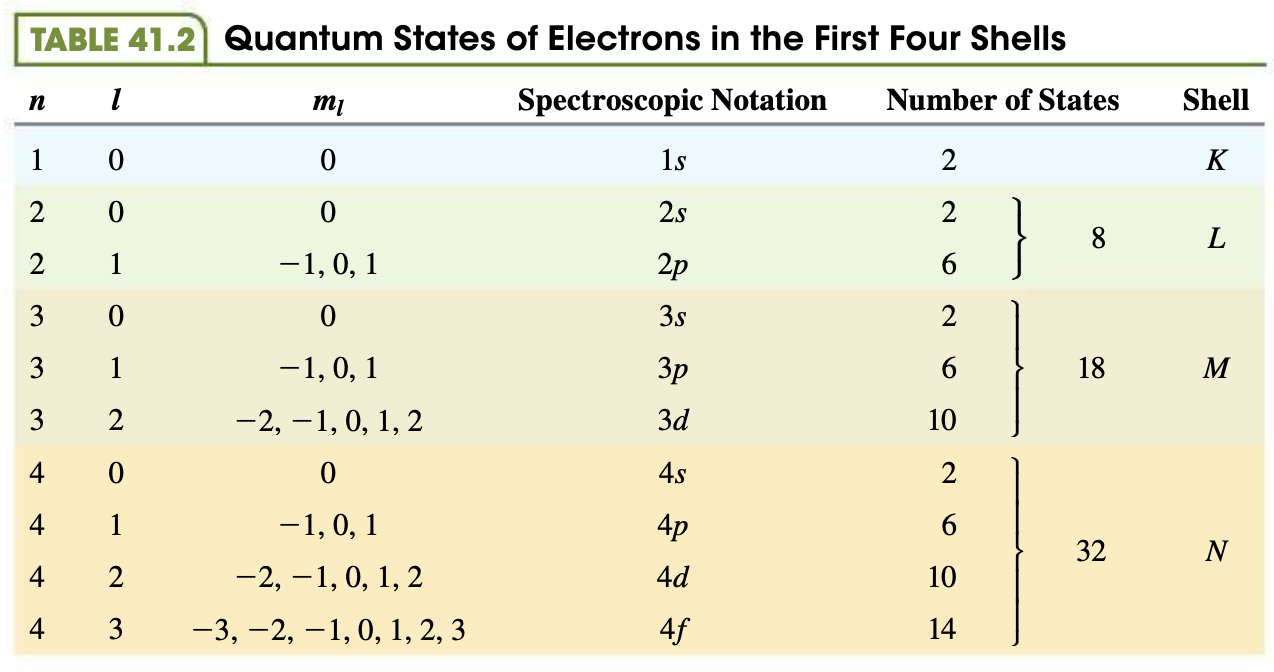
\includegraphics[scale=0.516]{shell-states}

\begin{itemize}
  \item The number of electrons permitted in each subshell is given by $2 (2 l + 1)$.

  \item The number of electrons permitted in each shell is given by $2 n^2$.

  \item The Pauli exclusion principle can be used to determine the ground state of an element with atomic number $Z$ by filling the lowest energy level electron positions from $1 s$ onwards. This can be represented as a sequence \begin{align*}
           & 1 s               \\
           & 1 s^2             \\
           & 1 s^2 2 s         \\
           & 1 s^2 2 s^2       \\
           & 1 s^2 2 s^2 2 p   \\
           & 1 s^2 2 s^2 2 p^2 \\
           & 1 s^2 2 s^2 2 p^3 \\
           & 1 s^2 2 s^2 2 p^4 \\
           & 1 s^2 2 s^2 2 p^5 \\
           & 1 s^2 2 s^2 2 p^6 \\
           & \qquad \vdots
        \end{align*} where superscripts indicate the number of electrons in that position.

  \item This pattern continues as expected until the $M$ and $N$ shells ($n = 3$ and $n = 4$) where some electrons go into the $4 s$ subshell instead of the $3 d$ subshell.

  \item Gauss's law tells us that if the charge distribution within an atom is spherically symmetrical (as in the central-field approximation), the electric field at radius $r$ is given by $Q_\text{encl} / 4 \pi \epsilon_0 r^2$. As you move from inner to outer shells, $Q_\text{encl}$ becomes less positive as electrons closer to the nucleus are \textbf{screening} some of its positive charge.

  \item From the view of electrons in outer shells, the atomic number of the atom is effectively reduced. The energy of an electron in shell $n$ is \[E_n = -\frac{Z_\text{eff}^2}{n^2} (\qty{13.6}{eV})\] where $Z_\text{eff}$ is the \textbf{effective atomic number} it experiences as a result of screening.

  \item An electron's $l$ value determines how many maxima are present in its wave function and how much ``time'' it spends at various distances from the nucleus. This means it determines $Z_\text{eff}$ and thus the electron's energy level.

  \item When electrons strike a metal target, their deceleration results in x-rays being emitted (bremsstrahlung or braking radiation). The type of metal determines the wavelengths that are emitted. There are peaks in radiation intensity at particlar wavelengths that change with the metal.

  \item The most intense peak is called the $K_\alpha$ line and its frequency is given by \textbf{Moseley's law} \[f = (\qty{2.48e15}{Hz}) (Z - 1)^2.\]
\end{itemize}

\section{Molecules and Condensed Matter}

\subsection{Types of Molecular Bonds}

\begin{itemize}
  \item An \textbf{ionic bond} is an interaction between oppositely charged ionized \\ atoms. One atom loses one or more electrons which requires energy — the \textbf{ionization energy} of the atom. The nucleus of the other atom is ineffectively screened by its electrons, attracting the free electrons and releasing energy — the \textbf{electron affinity} of the atom.

  \item The difference between the ionization energy and the electron affinity is the amount of energy required to create well-separated ions.

  \item The two oppositely charged ions are attracted to each other and move to an equilibrium position, releasing energy in the process. The difference between this energy and the amount of energy required to create well-separated ions is the \textbf{binding energy} of the molecule — the amount of energy required to dissociate the molecule into separate neutral atoms.

  \item A \textbf{covalent bond} is an interaction where two atoms share a pair of electrons between them. The attraction between the electrons and nuclei is great enough to overcome the repulsion between the electrons and between the nuclei.

  \item For many molecules, the sharing of electrons allows each atom to attain a full valence shell, e.g. in $\text{H}_2$ the two hydrogen atoms gain an electron, filling their first shell.

  \item Because the wave functions of the electrons overlap, the Pauli exclusion principle demands they have opposite spins. This means that only two electrons can participate in a covalent bond, however an atom with multiple electrons in its outermost shell can participate in multiple covalent bonds.

  \item Ionic and covalent bonds, with typical bond energies of $1$ to $\qty{5}{eV}$, are called \textbf{strong bonds}. There are also two kinds of weaker bonds: \textbf{van der Waals bonds} that are a result of fluctuating charge distributions and the resulting induced electric dipole momentts, and \textbf{hydrogen bonds} that occur when an $\text{H}^+$ ion (a bare proton) is inserted between two atoms causing them to polarize.
\end{itemize}

\subsection{Molecular Spectra}

\begin{itemize}
  \item Molecules have energy levels that are associated with rotation of a molecule as a whole and with vibration of the atoms relative to each other. Transitions between rotational and vibrational levels result in \textbf{molecular spectra}.

  \item The rotational energy levels of a diatomic molecule are \[E_l = l (l + 1) \frac{\hbar^2}{2 I}\] where $l$ is the \textbf{rotational quantum number} and can have values $l = 0, 1, 2, \ldots$, \[I = m_r r_0^2,\] \[m_r = \frac{m_1 m_2}{m_1 + m_2},\] and $r_0$ is the distance between the centres of the molecule's two atoms.

  \item Molecules aren't completely rigid. It's more accurate to model them as connected by a spring of constant $k'$. Then they can have vibrational energy levels given by \[E_n = \left( n + \frac{1}{2} \right) \hbar \sqrt{\frac{k'}{m_r}}\] where $n$ is the \textbf{vibrational quantum number} and can have values $n = 0, 1, 2, \ldots$.

  \item When rotational and vibrational energies are combined, the energy levels are \[E_{nl} = l (l + 1) \frac{\hbar^2}{2 I} + \left( n + \frac{1}{2} \right) \hbar \sqrt{\frac{k'}{m_r}}.\]

  \item To conserve angular momentum, when a photon is emitted $l$ must change by $\pm 1$.

  \item If the vibrational level changes, $n$ must increase by $1$ if a photon is absorbed and decrease by $1$ if a photon is emitted.
\end{itemize}

\subsection{Structure of Solids}

\begin{itemize}
  \item The term condensed matter refers to both solids and liquids.

  \item In condensed matter atoms attract each other until their outer electron clouds overlap, thus the distance between the centres of atoms is about the same as the diameter of the atoms themselves.

  \item \textbf{Crystalline solids} are solids with long-range order, i.e. a recurring pattern of atomic positions that occurs over many atoms.

  \item \textbf{Amorphous solids} are solids that have short- rather than long-range order.

  \item Liquids also only have short-range order.

  \item A \textbf{crystal lattice} is a repeating pattern of mathematical points that extends through space. There are 14 general types.
\end{itemize}

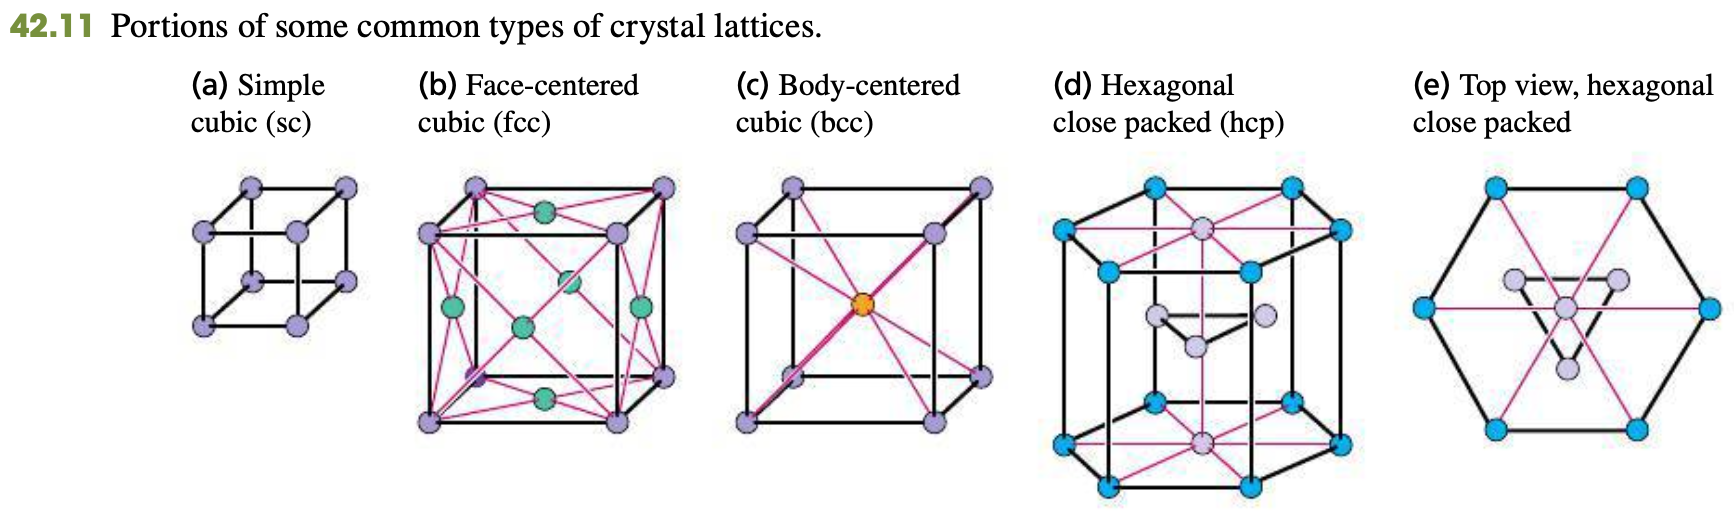
\includegraphics[scale=0.379]{crystal-lattices}

\begin{itemize}
  \item In a crystal structure, a single atom or a group of atoms is associated with each point. This atom or group of atoms is called the \textbf{basis} of the crystal structure.

  \item Ionic and covalent bonds are often responsible for the regular arrangement of atoms in a crystal.

  \item \textbf{Metallic crystals} are crystals in which one or more of the outermost electrons of each atom become detached, leaving a positive ion. The electrons are free to move through the crystal. This is what gives metals their high electrical and thermal conductivities.
\end{itemize}

\subsection{Energy Bands}

\begin{itemize}
  \item If you have a large number of identical atoms far enough apart that they don't interact, the energy level diagram of the system as a whole looks like that of an individual atom. If you gradually move the atoms closer together their wave functions begin to distort, particularly those of the outer or \textbf{valence electrons}. This distortion changes the energy levels of individual electrons — some up, some down — changing the energy level diagram. Because there are a large number of atoms and thus electrons, what started as a sharp line on the system's energy level diagram becomes an \textbf{energy band}.

  \item The highest band that is completely filled with electrons, i.e. there are electrons associated with all energy levels within the band, is called the \textbf{valence band}.

  \item The band above the valence band is called the \textbf{conduction band}.

  \item Insulators have a large gap between their valence and conduction bands, i.e. electrons must be given a large amount of energy to move to a higher energy level (dielectric breakdown).

  \item Semiconductors have a smaller gap between their valence and conduction bands meaning electrons must be given a smaller amount of energy to move to a higher energy level and this can come in the form of thermal energy. This is why semiconductors' resistance decreases with temperature.

  \item Conductors have a partially filled conduction band so only a very small amount of energy is required to move an electron to a higher energy level.
\end{itemize}

\subsection{Free-Electron Model of Metals}

\begin{itemize}
  \item The \textbf{free-electron model} assumes that detached electrons in a metal don't interact at all with its ions or other electrons but can't move past the surface of the metal, i.e. the potential energy function is $0$ within the metal and infinite at its surfaces.

  \item Sometimes we want to know the number of quantum states that have energies in a given range. The number of states per unit energy range is called the \textbf{density of states} denoted $g(E)$. Assuming the electrons are confined to a box of length $L$, then \[g(E) = \frac{(2 m)^{3 / 2} V}{2 \pi^2 \hbar^3} E^{1 / 2}\] where $E$ is the energy, $m$ is the mass of an electron, and $V$ is the volume of the box $L^3$.

  \item At absolute zero electrons want to be in as low of an energy state as possible, however the Pauli exclusion principle prevents them from being in the same state — this causes them to ``fill up energy states from the bottom.'' The energy level of the most energetic electron at absolute zero is known as the \textbf{Fermi energy at absolute zero $E_{F 0}$}.

  \item This behaviour lets us calculate $E_{F 0}$ using the formula for the number of energy states below energy $E$ \begin{align*}
          n       & = \frac{(2 m)^{3 / 2} V E^{3 / 2}}{3 \pi^2 \hbar^3}                            \\
          N       & = \frac{(2 m)^{3 / 2} V E_{F 0}^{3 / 2}}{3 \pi^2 \hbar^3}                      \\
          E_{F 0} & = \frac{3^{2 / 3} \pi^{4 / 3} \hbar^2}{2 m} \left( \frac{N}{V} \right)^{2 / 3} \\
                  & = \frac{3^{2 / 3} \pi^{4 / 3} \hbar^2 n^{2 / 3}}{2 m}                          \\
        \end{align*} where $n = N / V$ is the number of free electrons per unit volume or the \textbf{electron concentration}.

  \item The \textbf{Fermi-Dirac distribution} gives the probability that a given state is occupied by an electron \[f(E) = \frac{1}{e^{(E - E_F) / k T} + 1}\] where $E$ is the energy of the state and $E_F$ is the \textbf{Fermi energy}. We can use $E_F = E_{F0}$ at absolute zero or for metals.

  \item To calculate the number of electrons $d N$ in a given energy range $d E$ we must multiply the number of states in that range by the probability that each state is occupied \[d N = g(E) f(E) \,d E = \frac{(2 m)^{3 / 2} V E^{1 / 2}}{2 \pi^2 \hbar^3} \frac{1}{e^{(E - E_F) / k T} + 1} \,d E.\]

  \item At absolute zero, the average free electron energy is \[E_\text{av} = \frac{3}{5} E_{F 0}.\]
\end{itemize}

\subsection{Semiconductors}

\begin{itemize}
  \item A \textbf{semiconductor} has electrical resistivity that is intermediate between those of good conductors and good insulators. The gap between the valence and conduction bands is typically small which makes the resistivity very sensitive to temperature.

  \item When an electron gains enough energy to be removed from a covalent bond and move to the conduction band it leaves a vacancy or \textbf{hole} behind. Electrons in the valence band can then move into this hole. When an electric field is applied, electrons move in the opposite direction but holes move in the same direction, acting as positive charge carriers. This conductivity is called \textbf{intrinsic conductivity} and the material an \textbf{i-type semiconductor}.

  \item In a pure or \textbf{intrinsic} (i.e. not doped) semiconductor, conduction-band electrons and valence-band holes are always present in equal numbers because it takes one electron to make one hole.

  \item Mixing a different element with the semiconductor to change its composition is called \textbf{doping}.

  \item Doping a semiconductor with an element that has an additional electron in its valence shell (e.g. doping silicon with arsenic) means there is an excess of loosely bound electrons that can easily move to the conduction band. These electrons have an energy just below the bottom of the conduction band at the \textbf{donor level}. The impurity atom that is reponsible for this is called the \textbf{donor}. This is called an \textbf{n-type semiconductor} — the n referring to the fact that the majority of the charge carriers are negative.

  \item Doping a semiconductor with an element that has one fewer electron in its valence shell (e.g. doping silicon with boron) means there are holes in the crystal lattice and electrons in the valence shell can move around. The electrons in these holes have an energy just above the top of the valence band at the \textbf{acceptor level}. The impurity atom that is responsible for this is called the \textbf{acceptor}. This is called a \textbf{p-type semiconductor} — the p referring to the fact that the majority of the charge carriers are positive.
\end{itemize}

\subsection{Semiconductor Devices}

\begin{itemize}
  \item When a thin slab of semiconductor is irradiated with an electromagnetic wave whose photons have at least as much energy as the band gap between the valence and conduction bands, an electron in the valence band can absorb a photon and jump to the conduction band. This reduces the resistivity of the material. This is known as a photocell and is used to measure light intensity.

  \item A \textbf{p-n junction} is the boundary between a p-type semiconductor and an n-type semiconductor. When the p side is at a higher potential than the n side (\textbf{forward bias}), holes easily move from p to n and electrons easily move from n to p, giving a current. When the potential difference is reversed (\textbf{reverse bias}) there are very few electrons that can flow from p to n and very few holes that can flow from n to p, giving very little current. This is a \textbf{diode}.

  \item In a p-n junction there is diffusion between the p and n sides. Some holes from the p side move to the n side, and some electrons from the n side move to the p side. This makes the p side of the junction slightly negatively charged and the n side slightly positively charged. This results in an electric field that prevents further diffusion.

  \item When there is a forward bias (i.e. the p side is at a higher potential than the n side and there is an electric field from the p side to the n side) the holes and electrons have enough potential energy to jump the potential gap — this establishes a current. However the voltage needs to be greater than the potential difference between the two sides.

  \item The current through a p-n junction is \[I = I_S (e^{e V / k T} - 1)\] where $I_S$ is the saturation current (the maximum current in the reverse direction), the first $e$ is Euler's number, the second $e$ is the charge of an electron, and $V$ is the voltage.

  \item Light-emitting diodes (LEDs) are p-n junctions. When the diode is forward biased, holes move from the p region to the junction and electrons move from the n region to the junction. They combine in the junction, meaning the electron falls from the conduction band to the valence band and releases a photon with that amount of energy. The wavelength and thus colour of the photons are determined by the size of the band gap.

  \item The reverse of the above (the photovoltaic effect) is used to create solar cells. Electrons in the junction absorb photons creating electron-hole pairs. Those pairs are then separated by the recombination electric field, generating a current.
\end{itemize}

\section{Nuclear Physics}

\subsection{Properties of Nuclei}

\begin{itemize}
  \item The number of protons in a nucleus is called its \textbf{atomic number ($Z$)}.

  \item The number of neutrons in a nucleus is called its \textbf{neutron number ($N$)}.

  \item A \textbf{nucleon} is a neutron or a proton.

  \item The \textbf{nucleon number} of a nucleus is the number of nucleons it contains.

  \item The nucleon number is also called the \textbf{mass number} \[A = Z + N\] because it's the nearest whole number to the mass of the nucleus measured in atomic mass units (u) where \[\qty{1}{u} = \qty{1.660538921e-27}{kg}.\]

  \item The radius of an nucleus is \[R = R_0 A^{1 / 3}\] where \[R_0 = \qty{1.2e-15}{m} = \qty{1.2}{fm}\] and $A$ is the nucleon number.

  \item A nucleus's mass is proportional to $A$ and its volume is proportional to $R^3 = A$ so its density is constant. This means that all nuclei have approximately the same density.

  \item A particular combination of $Z$ and $N$ values is called a \textbf{nuclear species} or a \textbf{nuclide}. It's possible for different nuclides to have the same mass number.

  \item Nuclides that have the same number of protons ($Z$) but differenet numbers of neutrons ($N$) are called \textbf{isotopes}. They both represent the same element but have slightly different physical properties.

  \item The notation for nuclides is $^A_Z \text{El}$ or $^A \text{El}$ because $Z$ can be determined from the name of the element.

  \item Like electrons, nucleons are spin-$\frac{1}{2}$ particles.

  \item The magnitude of the spin angular momentum of a nucleon is \[S = \sqrt{\frac{1}{2} \left( \frac{1}{2} + 1 \right)} \hbar = \sqrt{\frac{3}{4}} \hbar\] and the $z$-component is \[S_Z = \pm \frac{1}{2} \hbar.\]

  \item The total orbital angular momentum of a nucleus has magnitude \[J = \sqrt{j (j + 1)} \hbar\] and $z$-component \[J_z = m_j \hbar, \,m_j = -j, -j + 1, \ldots, j - 1, j\] where $j$ is the \textbf{nuclear spin}.

  \item When the total number of nucleons $A$ is even, $j$ is an integer. When it's odd, $j$ is a half-integer.

  \item When $Z$ and $N$ are both even, $J = 0$.

  \item The \textbf{nuclear magneton} is to nucleons what the Bohr magneton is to electrons (the quanta of magnetic moment) \[\mu_n = \frac{e \hbar}{2 m_p} = \qty{5.05078e-27}{J/T} = \qty{3.15245e-8}{eV/T}.\]

  \item The magnitude of the $z$-component of spin magnetic moment of a proton is \[|\mu_n|_\text{proton} = 2.7928 \mu_n\] and it is parallel to the spin angular momentum.

  \item The magnitude of the $z$-component of the spin magnetic moment of a neutron is \[|\mu_n|_\text{neutron} = 1.9130 \mu_n\] and it is antiparallel to the spin angular momentum.

  \item Because a nucleus has a magnetic moment, there is an interaction energy \[U = -\boldsymbol{\mu} \cdot \mathbf{B}\] when it is placed in an external magnetic field. The component of the magnetic moment in the direction of the magnetic field $\mu_z$ is quantized so a series of energy levels results from this interaction.

  \item The magnetic moment of the nucleus causes a magnetic field. The interaction of electrons with this magnetic field results in \textbf{hyperfine structure} — the additional splitting of energy levels and spectra.
\end{itemize}

\subsection{Nuclear Binding and Nuclear Structure}

\begin{itemize}
  \item Because energy must be added to a nucleus to separate it into its individual nucleons, the total rest energy of the separated nucleons $E_0$ is greater than the rest energy of the nucleus.

  \item The energy the must be added to separate the nucleons is called the \textbf{binding energy $E_B$} thus the rest energy of the nucleus is $E_0 - E_B$.

\item Using the mass-energy equivalence $E = m c^2$ we can calculate the binding energy $E_B$ as the difference in mass between the separated nucleons and the nucleus \[E_B = (Z M_H + N m_n - ^A_Z M) c^2\] where $M_H$ is the mass of a hydrogen atom \[M_H = \qty{1.007825}{u},\] $m_n$ is the mass of a neutron \[m_n = \qty{1.008665}{u},\] $^A_Z M$ is the mass of a neutral atom containing the nucleus in question, and \[c^2 = \qty{931.5}{MeV/u}.\]

  \item An important measure of how tightly a nucleus is bound is the \textbf{binding energy per nucleon} $E_B / A$.

  \item The mass of a nucleus is always smaller than the mass of its constituent nucleons by $\Delta M = E_B / c^2$. This is called the \textbf{mass defect}.

  \item The force that binds neutrons and protons together in the nucleus is an example of the strong interaction. In this context it's called the \textbf{nuclear force}.

  \item The nuclear force…

        \begin{itemize}
          \item Does not depend on charge. Neutrons and protons are both bound.

          \item Exhibits ``saturation'', i.e. an individual nucleon only interacts with a few of its neighbours.

          \item Has a short range (on the order of $10^{-15} \,\unit{m}$) but within that range it's much stronger than electric forces.

          \item Favors binding pairs of neutrons or protons with opposite spins and of pairs of pairs (i.e. a pair of neutrons or a pair of protons, each pair having opposite spins).
        \end{itemize}

  \item The \textbf{liquid-drop model} for nuclear structure estimates the binding energy of a nucleus as \[E_B = C_1 A - C_2 A^{2 / 3} - C_3 \frac{Z (Z - 1)}{A^{1 / 3}} - C_4 \frac{(A - 2 Z)^2}{A} \pm C_5 A^{-4 / 3}\] where \begin{align*}
          C_1 & = \qty{15.75}{MeV}  \\
          C_2 & = \qty{17.80}{MeV}  \\
          C_3 & = \qty{0.7100}{MeV} \\
          C_4 & = \qty{23.69}{MeV}  \\
          C_5 & = \qty{39}{MeV}
        \end{align*} and the $C_5$ term is positive if both $Z$ and $N$ are even, negative if they're both odd, and zero otherwise.

  \item The \textbf{semiempirical mass formula}, derived from the liquid-drop model, can be used to estimate the mass of any neutral atom \[^A_Z M = Z M_H + N m_n - \frac{E_B}{c^2}.\]

  \item The \textbf{shell model} for nuclear structure assumes a spherically symmetric potential energy function (similar to the central-field approximation for electrons).

  \item As neutrons and protons are also spin-$\frac{1}{4}$ particles, the Pauli exclusion principle prevents any two from occupying the same state within a nucleus. Like the noble gases, this results in certain \textbf{magic numbers} of neutrons and/or protons that result in particularly high binding energies and thus stable nuclei. The numbers are 2, 8, 20, 28, 50, 82, and 126.
\end{itemize}

\subsection{Nuclear Stability and Radioactivity}

\begin{itemize}
  \item Among ~2500 known nuclides, fewer than 300 are stable. The others are unstable and decay into other nuclides by emitting electromagnetic radiation and particles, a process called \textbf{radioactivity}.

  \item A \textbf{Segrè chart} has neutron number on the $y$-axis, proton number on the $x$-axis, and plots points where the combination results in a stable nuclide.

  \item Each value of the mass number $A$ typically only has 2 or 3 associated stable nuclides.

  \item Most stable nuclides have an even number of neutrons and/or protons. Only 3 have odd numbers of both.

  \item The plot of stable nuclides forms a line slightly steeper than the $N = Z$ line. Nuclides in the region to the left have too many neutrons and convert them to protons via $\beta^-$ decay. Nuclides in the region to the right have too many protons and electric repulsion causes the atom to split.

  \item \textbf{Alpha decay} occurs when an unstable nuclide emits an \textbf{alpha particle}: a $^4 \text{He}$ nucleus. This occurs principally with nuclei that are too large to be stable. When a nucleus emits an alpha particle its $N$ and $Z$ values both decrease by 2.

  \item Alpha decay is possible whenever the mass of the original neutral atom is greater than the sum of the masses of the final neutral atom and a neutral $^4_2 \text{He}$ atom. The difference in mass is converted into the kinetic energy of the alpha particle and daughter nucleus (both may be moving due to conservation of momentum).

  \item The original nucleus is called the \textbf{parent nucleus} and the remaining nucleus is called the \textbf{daughter nucleus}.

  \item Sometimes the parent nucleus decays to an excited state of the daughter nucleus which then emits an additional photon.

  \item Alpha particles are emitted at high speeds (typically a few percent of the speed of light), but because of their charge and mass they can typically only travel a few centimeters in air or a small fraction of a millimeter in solids.

  \item In \textbf{beta-minus ($\boldsymbol{\beta}^-$) decay}, a neutron changes into a proton, a $\beta^-$ particle (an electron), and an antineutrino $\overline{\nu}_e$. The nucleus's neutron number $N$ decreases by one and its proton number $Z$ increases by one.

  \item $\beta^-$ particles (electrons) are emitted at very high speeds — up to 0.9995 of the speed of light — so their motion is highly relativistic.

  \item The antineutrino is the antiparticle of the neutrino. It has zero charge, very small mass, and is spin-$\frac{1}{2}$.

  \item $\beta^-$ decay can occur whenever the mass of the original neutral atom is larger than that of the final atom.

  \item Because there are three products in $\beta^-$ decay, the energy can be shared in many different ways while still converving energy and momentum. This makes it impossible to predict precisely how the energy will be shared, incontrast with $\alpha$ decay where only two products mean the energy and momenta can be uniquely determined.

  \item In \textbf{beta-plus ($\boldsymbol{\beta}+$) decay}, a proton changes into a neutron, a $\beta+$ particle (a positron), and a neutrino $\nu_e$. The nucleus's neutron number $N$ increases by one and its proton number $Z$ decreases by one.

  \item $\beta^+$ decay can occur whenever the mass of the original neutral atom is at least two electron masses larger than that of the final atom.

  \item In \textbf{electron capture}, an orbital electron (typically in the $K$ shell) can combine with a proton in the nucleus to form a neutron and a neutrino. The neutron remains in the nucleus and the neutrino is emitted. The nucleus's neutron number increases by one and its proton number decreases by one.

  \item Electron capture can occur whenever the mass of the original neutral atom is larger than that of the final atom.

  \item Like electrons, the internal energy of nuclei is quantized and they have a ground state. However because of the great strength of nuclear interactions, excitation energies of nuclei are much greater than those of electrons.

  \item When a nucleus is in an excited state it can decay to its ground state by emitting a high-energy photon or \textbf{gamma ($\boldsymbol{\gamma}$) ray}. This process is called \textbf{gamma ($\boldsymbol{\gamma}$) decay}.

  \item In both $\alpha$ and $\beta$ decay the $Z$ value of the nucleus changes. In $\gamma$ decay it doesn't.

  \item When an unstable nucleus decays, the daughter nucleus may also be unstable and itself decay. This results in a series of decays until a stable configuration is reached.
\end{itemize}

\subsection{Activities and Half-Lives}

\begin{itemize}
  \item If you have a number of unstable nuclei $N(t)$ they will decay over time and the number will decrease, i.e. $d N(t) / d t$ is negative.

  \item The number of nuclei decaying per unit interval $-d N(t) / d t$ is called the \textbf{activity} or \textbf{decay rate} of the specimen and is proportional to the remaining number of nuclei present \[-\frac{d N(t)}{d t} = \lambda N(t)\] where $\lambda$ is the \textbf{decay constant}.

  \item If $\lambda$ is large the sample decays quickly, if it's small it decays slowly.

  \item The number of remaining nuclei at time $t$ is \[N(t) = N_0 e^{-\lambda t}\] where $N_0$ is the number of nuclei present at $t = 0$.

  \item The \textbf{half-life} of a sample is the amount of time required for half of its nuclei to decay \[T_{1 / 2} = \frac{\ln 2}{\lambda} = \frac{0.693}{\lambda}.\]

  \item The \textbf{(mean) lifetime} of an unstable nucleus is proportional to its half-life \[T_\text{mean} = \frac{1}{\lambda} = \frac{T_{1 / 2}}{\ln 2} = \frac{T_{1 / 2}}{0.693}.\]

  \item A common unit of radioactive activity is the \textbf{curie} where \[\qty{1}{Ci} = \num{3.70e10} \text{ decays/s}.\]

  \item The SI unit of activity is the \textbf{becquerel} where \[\qty{1}{Bq} = 1 \text{ decay/s}.\]
\end{itemize}

\subsection{Biological Effects of Radiation}

\begin{itemize}
  \item The \textbf{absorbed dose} of radiation is the amount of energy delivered by the radiation per unit mass of living tissue.

  \item The unit of absorbed dose is the gray where \[\qty{1}{Gy} = \qty{1}{J/kg}.\]

  \item Another common unit is the rad where \[\qty{1}{rad} = \qty{0.01}{J/kg} = \qty{0.01}{Gy}.\]

  \item \textbf{Ionizing radiation} is radiation that has enough energy to ionize atoms, i.e. strip them of their electrons.

  \item Different types of radiation have different effects on living tissue. The \textbf{relative biological effectiveness (RBE)} or \textbf{quality factor (QF)} is a number associated with each type of radiation that quantifies the scale of its effects.
\end{itemize}

\begin{center}
  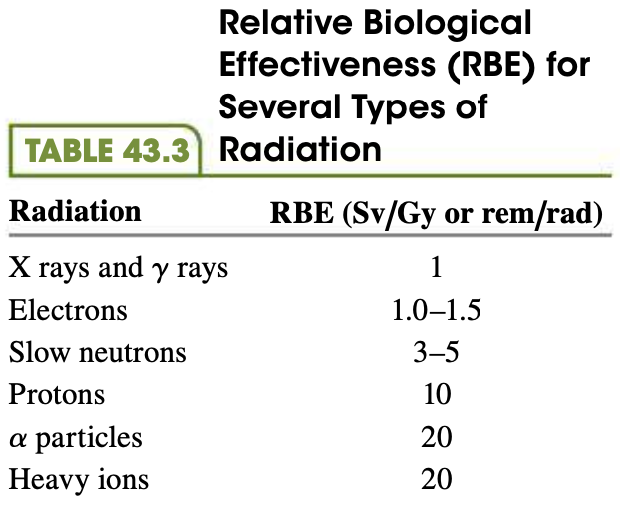
\includegraphics[scale=0.43]{rbe}
\end{center}

\begin{itemize}
  \item The biological effects of radiation can be quantified as the product of the absorbed dose (in $\unit{Gy}$ or $\unit{rad}$) and the RBE of the radiation. This is called the \textbf{biologically equivalent dose} or \textbf{equivalent dose}.

  \item The units of equivalent dose are sieverts ($\unit{Sv}$) when the absorbed dose is measured in gray, and rem ($\unit{rem}$) when it's measured in rad.

  \item While the units of gray and sieverts are both equivalent to $\unit{J/kg}$, the former is used to communicate the quantity of an absorbed dose while the latter is used to communicate the biological effects of an absorbed dose.
\end{itemize}

\subsection{Nuclear Reactions}

\begin{itemize}
  \item A \textbf{nuclear reaction} is the rearrangement of nuclear components that result from a bombardment by a particle rather than a spontaneous natural process.

  \item Nuclear reactions are subject to several conservation laws: charge, momentum, angular momentum, energy, and the total number of nucleons. Note that the number of neutrons and protons may not be conserved as they can change into each other in $\beta$ decay.

  \item In general, nuclear reactions are not elastic collisions and the total initial mass does not equalt the total final mass.

  \item By the mass-energy equivalence, the difference in mass before and after the reaction corresponds to the \textbf{reaction energy}. If initial particles $A$ and $B$ interact to produce particles $C$ and $D$, then the reaction energy is \[Q = (M_A + M_B - M_C - M_D) c^2.\] To balance the electrons, the neutral atomic masses are used.

  \item When the reaction energy is positive, the total mass decreases and the total kinetic energy increases. This is called an \textbf{exoergic reaction}.

  \item Even though energy is released in an exoergic reaction, the initial kinetic energies must be great enough for the particles to overcome their electric repulsion unless they tunnel.

  \item When the reaction energy is negative, the total mass increases and the total kinetic energy decreases. This is called an \textbf{endoergic reaction}.

  \item An endoergic reaction can't occur unless the initial kinetic energy in the centre of mass reference frame is at least as great as $|Q|$. This is called the \textbf{threshold energy}.
\end{itemize}

\subsection{Nuclear Fission}

\begin{itemize}
  \item \textbf{Nuclear fission} is a decay process in which an unstable nucleus splits into two fragments of comparable mass (\textbf{fission fragments}).

  \item Fission resulting from neutron absorption is called \textbf{induced fission}.

  \item Some nuclides also undergo \textbf{spontaneous fission} without neutron absorption but this is rare.

  \item Fission fragments typically have large kinetic energies. This is because they typically have much larger binding energies than the parent nucleus, resulting in lower rest energy and thus a release of energy during the reaction.

  \item Fission fragments are always unstable because their $N / Z$ ratio is too high. They typically turn into stable nuclides via a chain of $\beta^-$ decays.
\end{itemize}

\subsection{Nuclear Fusion}

\begin{itemize}
  \item In a \textbf{nuclear fusion} reaction, two or more small light nuclei come together, or fuse, to form a larger nucleus. These reactions release energy because the binding energy per nucleon after the reaction is greater than before.

  \item The binding energy per nucleon increases until around $A = 60$, so the mass numbers of the initial nuclei must add to less than $60$.
\end{itemize}

\section{Particle Physics and Cosmology}

\subsection{Fundamental Particles - A History}

\begin{itemize}
  \item In particle physics, a photon is denoted by the Greek symbol gamma $\gamma$.

  \item A \textbf{positron} is a particle with the same mass as an electron but a positive charge.

  \item Electron-positron pairs are produced during high-energy collisions of \\ charged particles or $\gamma$ rays with matter. This process is called \textbf{$\mathbf{e^+ e^-}$ pair production}.

  \item The minimum energy required for pair production is the rest energy of the two particles $2 m_e c^2 = \qty{1.022}{MeV}$.

  \item When an electron and a positron collide both particles disappear, and two (or sometimes three) photons appear with total energy greater than the rest energy of the original particles. this process is called \textbf{$\mathbf{e^+ e^-}$ pair annihilation}.

  \item It's impossible for a single photon to appear after pair annihilation as that wouldn't conserve momentum.

  \item Particles that are related to another particle as the positron is to the electron are called \textbf{antiparticles}.

  \item Some particles (necessarily with neutral charge) are their own antiparticles, e.g. photons.

  \item The uncertainty principle $\Delta E \Delta t \ge \hbar / 2$ permits the creation of a \textbf{virtual photon} of energy $\Delta E$ as a force carrier providing it exists for no longer than $\Delta t$.
\end{itemize}

\subsection{Particle Accelerators and Detectors}

\begin{itemize}
  \item A \textbf{linear accelerator (linac)} accelerates particles in a straight line.

  \item A \textbf{cyclotron} accelerates particles by applying an electric field between two electrodes and causes them to move in a circle via a magnetic field.

  \item When a high-energy particle collides with a stationary target the products of the collision must have some motion to preserve momentum. This means not all kinetic energy is available to form new particle states. The energy that may be used is known as the \textbf{available energy}.

  \item If the particles involved in a collision are travelling at equal speeds in opposite directions, the centre of momentum frame is equal to the laboratory frame and available energy is maximised.

  \item The electromagnetic interaction is mediated by photons.

  \item Photons have spin $s = 1$ so the magnitude of spin angular momentum is $S = \sqrt{s (s + 1)} \hbar = \sqrt{2} \hbar$.

  \item The gravitational interaction is mediated by gravitons.

  \item Gravitons have spin $s = 2$ so the magnitude of spin angular momentum is $S = \sqrt{s (s + 1)} \hbar = \sqrt{6} \hbar$.

  \item The \textbf{strong interaction} is responsible for the nuclear force.

  \item The strong interaction is mediated by gluons, but can be more easily explained as being mediated by mesons.

  \item The strong interaction is roughly 100 times stronger than the electromagnetic interaction.

  \item The \textbf{weak interaction} is responsible for beta decay and other types of radioactive decays.
\end{itemize}

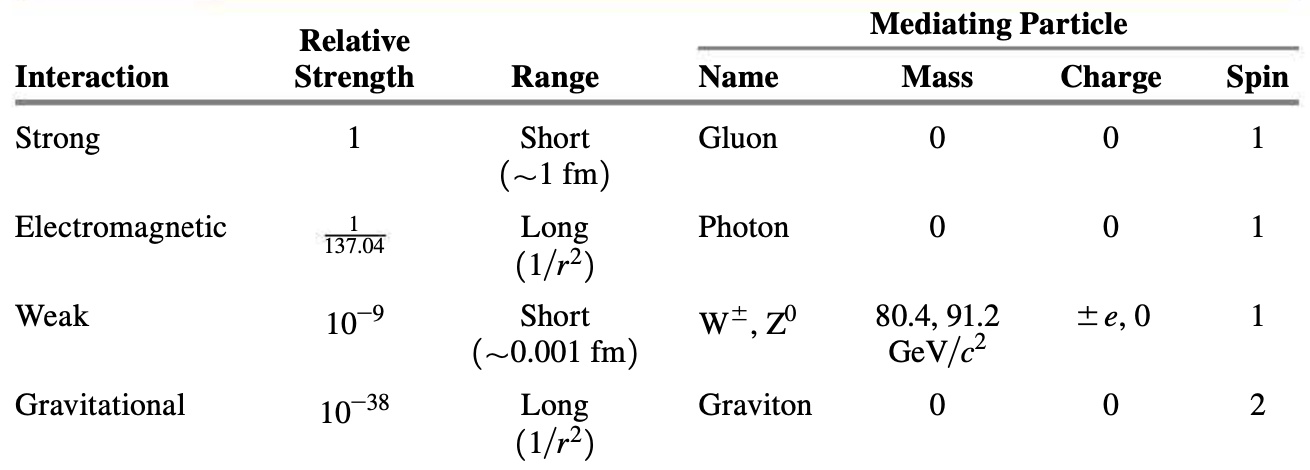
\includegraphics[scale=0.5]{interactions}

\begin{itemize}
  \item \textbf{Fermions} have half-integer spins, obey the exclusion principle, and obey the Fermi-Dirac distribution.

  \item \textbf{Bosons} have zero or integer spin, don't obey the exclusion principle (i.e. there's no limit to the number of bosons in a given quantum state), and obey the Bose-Einstein distribution instead of the Fermi-Dirac distribution.

  \item \textbf{Leptons} are elementary particles that don't undergo strong interactions and have spin $\frac{1}{2}$ (making them fermions). There are six leptons.
\end{itemize}

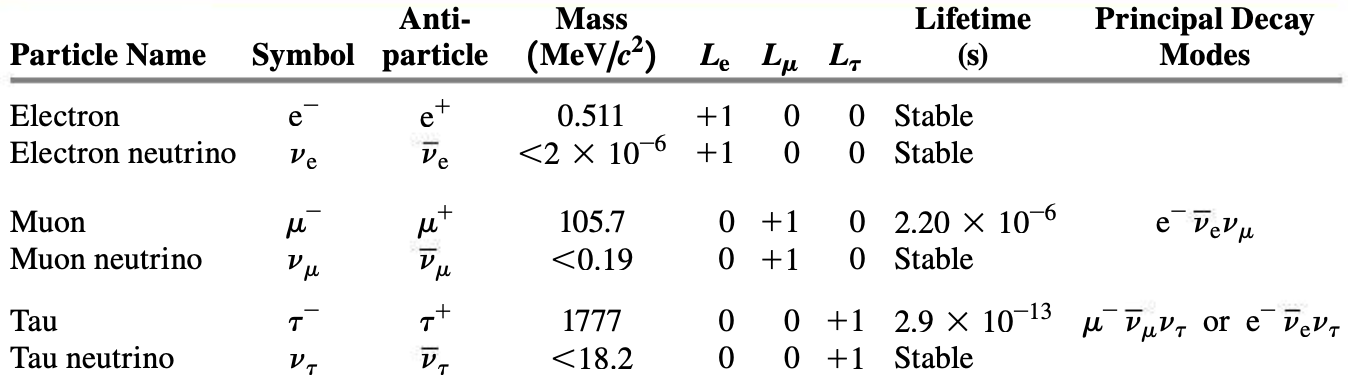
\includegraphics[scale=0.48]{leptons}

\begin{itemize}
  \item The leptons are assigned three \textbf{lepton numbers} $L_e$, $L_\mu$, and $L_\tau$. In all interactions, each lepton number is separately conserved.

  \item \textbf{Hadrons} are subatomic particles that undergo strong interactions.

  \item Hadrons can be further classified as \textbf{mesons} which have spin 0 or 1 and are thus bosons, and \textbf{baryons} which have half-integer spin and are thus fermions.

  \item Each baryon has \textbf{baryon number} $B = 1$ and each antibaryon has $B = -1$. In all interactions, the total baryon number is conserved.

  \item \textbf{Strangeness} is a property of particles. Strangeness is conserved in strong interactions but may change by zero or one unit in weak interactions.
\end{itemize}

\subsection{Quarks and Gluons}

\begin{itemize}
  \item Hadrons are comprised of spin-$\frac{1}{2}$ fermions called \textbf{quarks}.

  \item Each baryon is composed of three quarks.

  \item Each antibaryon is composed of three antiquarks.

  \item Each meson is composed of a quark-antiquark pair.

  \item There are several types of quarks with different charge, spin, baryon number, etc. Each subatomic particle composed of quarks has properties that are the sum of those of their constituent quarks.

  \item The attractive interaction among quarks are mediated by massless, spin-1 bosons called \textbf{gluons}.

  \item Quarks are fermions and are thus subject to the exclusion principle. This seems to forbid a baryon having multiple quarks of the same flavor. This can be explained by introducing the concept of \textbf{colour}.

  \item Each quark has a color: red, antired, blue, antiblue, green, or antigreen. Colour is always conserved and can change via the emission of gluons.
\end{itemize}

\setcounter{subsection}{5}
\subsection{The Expanding Universe}

\begin{itemize}
  \item Astronomical distances are often measured in \textbf{parsecs} ($\unit{pc}$). One parsec is the distance at which there is one-arcsecond ($1 / \ang{3600}$) angular separation between two objects $\qty{1.50e11}{m}$ apart (the average distance from the earth to the sun). A distance of $\qty{1}{pc}$ is equal to $\qty{3.26}{ly} = \qty{9.46e12}{km}$.

  \item The \textbf{Hubble law} states that the speed of recession $v$ of a galaxy is proportional to its distance $r$ from us \[v = H_0 r\] where \[H_0 = \qty{67.3}{km/(Mpc.s)} = \qty{2.18e-18}{s^{-1}}.\]

  \item The \textbf{cosmological principle} states that, on average, the universe looks the same from all locations.

  \item \textbf{Dark matter} is matter that doesn't emit electromagnetic radiation. It accounts for $5 \frac{1}{2}$ times more mass than luminous matter.

  \item \textbf{Dark energy} is an unknown form of energy that is thought to be causing the expansion of the universe to accelerate.
\end{itemize}

\subsection{The Beginning of Time}

\begin{itemize}
  \item
\end{itemize}

\end{document}